\onehalfspacing
\fancypagestyle{plain}{
	\fancyhf{}
	\rhead{\thepage}
	\renewcommand{\headrulewidth}{0pt}
	\renewcommand{\footrulewidth}{0pt}
}

\chapter{DISEÑO CONCEPTUAL}

\section{Caja Negra}

Como primer paso para el modelado del diseño conceptual, es fundamental delimitar las fronteras del proyecto y comprender los elementos del sistema fotovoltaico con los que este va a interactuar. Para ello, se emplea el diagrama de Black Box, el cual permite visualizar la operación del sistema en su nivel más alto de abstracción mediante la representación de sus entradas y salidas.

En la Figura \ref{fig:caja_negra} se presenta la abstracción funcional del sistema de inspección a nivel de caja negra, la cual define las fronteras del producto y su interacción con el entorno.

\begin{figure}[H]
	\captionsetup{justification=raggedright, singlelinecheck=false, labelsep=none}
	\caption[Abstracción funcional del sistema de inspección a nivel de caja negra.]{} 
	\textit{Abstracción funcional del sistema de inspección a nivel de caja negra.} \par\medskip
	
	\makebox[\textwidth][c]{ 
		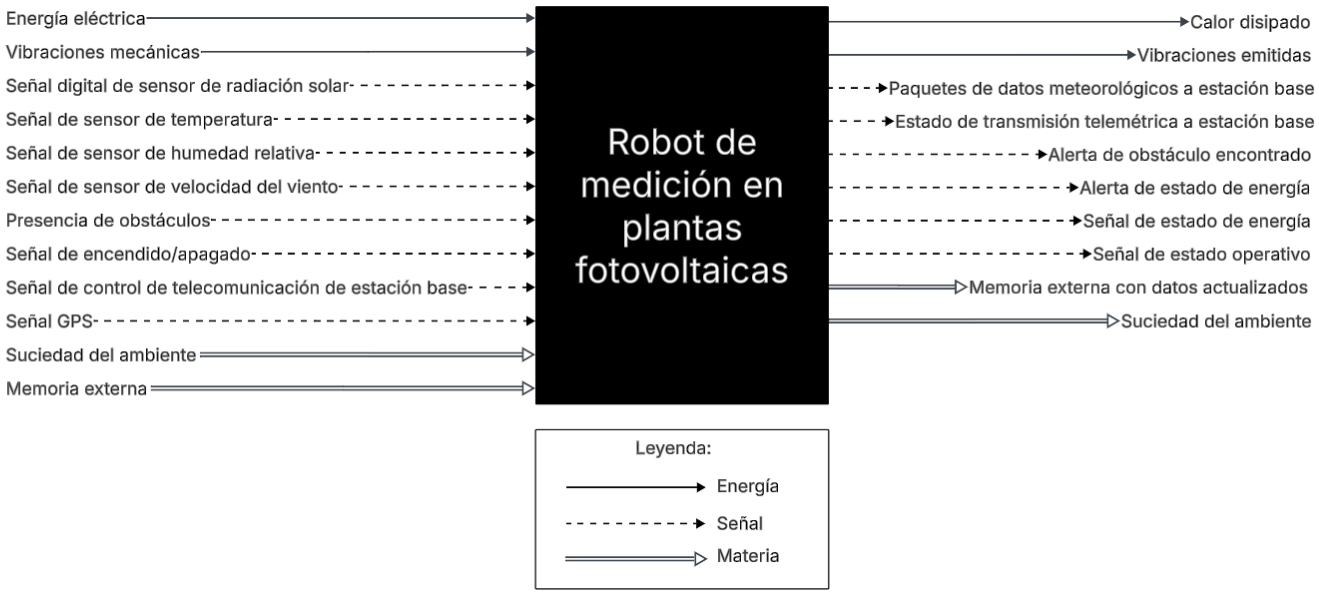
\includegraphics[width=1.2\textwidth]{Imagenes/A3_Blackbox_v7.png}
	} \par\medskip
	
	\raggedright
	\footnotesize \textit{Nota.} Elaboración propia.
	\label{fig:caja_negra}
\end{figure}

La función principal del sistema se define como: Transformar señales de instrumentación meteorológica externa, información espacial y comandos del usuario en paquetes de datos procesados con validez industrial y reportes de estado telemétrico.

Para cumplir con su objetivo, el sistema recibe flujos de energía de entrada compuestos por la energía eléctrica directa necesaria para su alimentación y las perturbaciones provenientes del terreno en forma de vibraciones mecánicas.

Simultáneamente, el sistema capta flujos de señales e información provenientes del entorno, las cuales incluyen la data climática (señal digital de sensor de radiación solar, señal de sensor de temperatura, señal de sensor de humedad relativa y señal de sensor de velocidad del viento), la señal GPS y la presencia de obstáculos; mientras que, desde el exterior, se introducen las instrucciones mediante la señal de encendido/apagado y la señal de control de telecomunicación de estación base.

Por otro lado, los flujos de materia que interactúan en las fronteras de entrada del sistema corresponden a la inserción física de la memoria externa y al ingreso inevitable de la suciedad del ambiente, propia de las instalaciones fotovoltaicas.

Como resultado de la transformación interna, el sistema entrega, como salidas útiles, un flujo de información compuesto por los paquetes de datos meteorológicos a estación base, el estado de transmisión telemétrica a estación base, las advertencias críticas de alerta de obstáculo encontrado y alerta de estado de energía, así como la señal de estado de energía y la señal de estado operativo requeridas para la interfaz local. Es importante destacar que estos flujos de comunicación, tanto de entrada como de salida, representan tramas de bytes estructuradas, garantizando la integridad y correcta interpretación de la telemetría.

A nivel de flujos de materia, el sistema depara la extracción de la memoria externa con datos actualizados, la cual contiene el respaldo físico de la información, y la evacuación o paso de la suciedad del ambiente.

Finalmente, como residuo del trabajo físico y computacional, el sistema libera al entorno flujos de energía en forma de calor disipado y vibraciones emitidas durante su desplazamiento continuo. Además, el sistema provee como salida un flujo de energía eléctrica para sensores meteorológicos, asegurando la alimentación y operatividad de la instrumentación externa.


\section{Estructura de Funciones}

A partir de la caja negra, se desarrolla la estructura de funciones (ver Anexo 2). En este esquema, la función principal del sistema se descompone en dominios, cada uno con bloques que describen las funciones elementales del robot, relacionando detalladamente los flujos internos de energía, materia y señales.

\subsection{Dominio de Energía}
El Dominio de Energía se encarga de la recepción, gestión y distribución del recurso eléctrico necesario para garantizar el funcionamiento de todos los subsistemas del robot, a través del siguiente flujo, ilustrado en la Figura \ref{Avance3_DomEnergia}:

\begin{itemize}
	\item \textbf{Recibir energía eléctrica:} Para esta función se evaluó el conector \textit{Plug Jack} DC, que permite una conexión lineal simple para corrientes medias; el conector de alta corriente XT60, el cual asegura una conexión física firme capaz de soportar las vibraciones mecánicas de un terreno irregular; y los contactos magnéticos, que facilitan un acople automático sin requerir exactitud cinemática, aunque son vulnerables a perder continuidad \citep{Salinas2025}.
	
	\item \textbf{Proteger sistema eléctrico:} Se analizó el fusible electrónico \textit{eFuse} por su corte rápido y posibilidad de restablecimiento automático, ideal para proteger la navegación de vehículos terrestres autónomos \citep{CN221163061U}; el disyuntor termomagnético, que ofrece una protección robusta ante cortocircuitos pero exige rearme manual; y el fusible cerámico de cartucho, una opción de bajo costo que requiere reemplazo físico tras activarse.
	
	\item \textbf{Gestionar energía eléctrica:} Las opciones contemplan la batería LiPO con \textit{Battery Management System} (BMS), destacada por sus altas tasas de descarga para superar obstáculos, pero con menor vida útil; la batería Li-Ion con BMS, que proporciona una alta densidad energética para asegurar la autonomía de operación del robot; y la batería NiMH con BMS, una alternativa muy estable frente a los riesgos térmicos de la intemperie solar, pero con menor densidad de energía que el resto \citep{XPower2024}.
	
	\item \textbf{Activar energía eléctrica:} Se consideró el relé de estado sólido, que permite la conmutación de potencia mediante señales de control sin desgaste de partes móviles; el contactor mecánico, útil para manejar los picos de corriente durante el arranque de los motores de tracción; y el seccionador rotativo manual, que actúa como un elemento de corte físico directo, obligatorio como método de parada \citep{Burriana5MW}.
	
	\item \textbf{Regular energía (Interfaz, Control/Comm., Sensores y Meteorología):} Se evaluó el regulador \textit{Shunt}, de diseño extremadamente simple pero térmicamente ineficiente al disipar el exceso de voltaje como calor; el regulador de bomba de carga (\textit{Charge pump}), útil para elevar o reducir voltajes en espacios reducidos pero limitado a bajas corrientes; y el regulador lineal LDO, que, aunque disipa calor, ofrece un voltaje de salida muy estable y con bajo ruido eléctrico.
	
	\item \textbf{Regular energía de Actuadores:} Para esta etapa crítica de regulación de potencia motriz se analizó el regulador lineal LDO, que entrega un voltaje limpio pero genera demasiada pérdida térmica frente a la alta demanda de los motores al escalar pendientes; el regulador de bomba de carga, de circuito compacto pero con capacidad de corriente insuficiente; y el convertidor \textit{Buck} DC-DC, que posee una alta eficiencia de conmutación energética para soportar el consumo dinámico del mecanismo de locomoción.
	
	\item \textbf{Energizar componentes y distribución interna:} Se propusieron las barras colectoras (\textit{Busbars}) para facilitar una distribución rígida y de alta corriente; el cable trenzado estándar, que aporta flexibilidad y bajo costo para el ruteo interno en la caja de control; y los conectores circulares roscados, que garantizan uniones impermeables y resistentes a las desconexiones causadas por la irregularidad de la topografía \citep{CN120057153A}.
\end{itemize}

\begin{figure}[H]
	\captionsetup{justification=raggedright, singlelinecheck=false, labelsep=none}
	
	\caption[Dominio de energía de la estructura de funciones.]{} 
	
	\textit{Dominio de energía de la estructura de funciones.} \par\medskip
	
	\makebox[\textwidth][c]{
		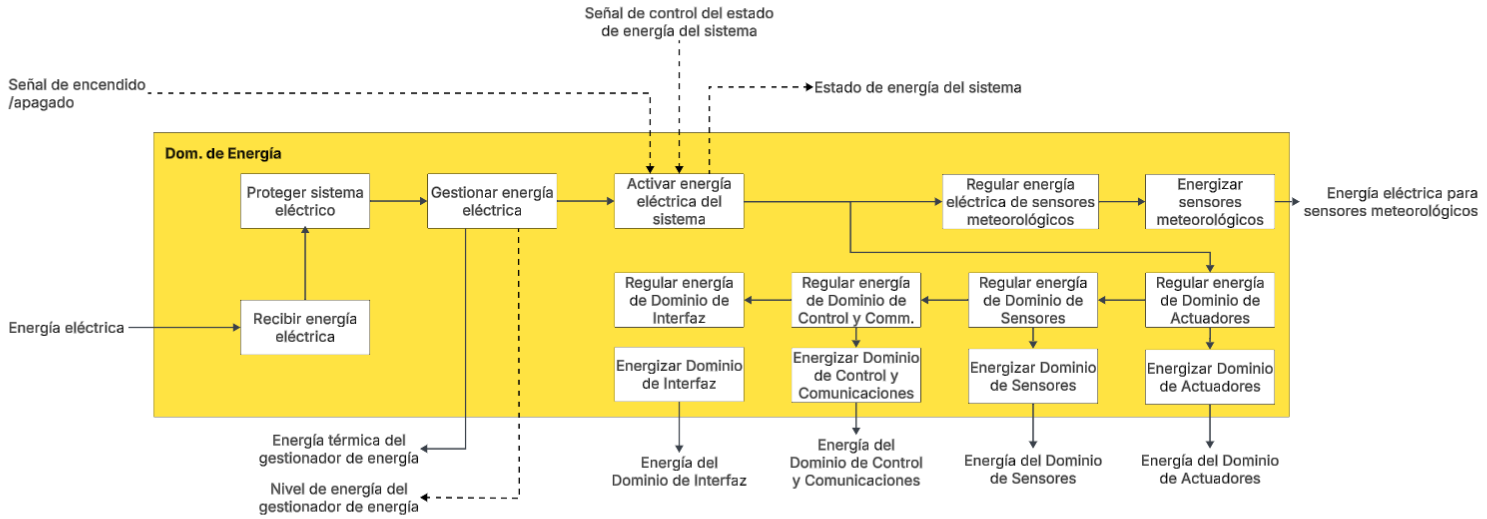
\includegraphics[width=1.2\textwidth]{Imagenes/A3_DominioEnergia.png}
	} \par\medskip
	
	\raggedright
	\footnotesize \textit{Nota.} Elaboración propia.
	\label{fig:Avance3_DomEnergia}
\end{figure}

\subsection{Dominio de Sensores}
El Dominio de Sensores actúa como el sistema de medición y detección del ambiente del robot, encargado de adquirir los estados físicos de los componentes y del entorno inmediato para su posterior procesamiento. Este dominio es alimentado de forma general por el flujo de energía del Dominio de Sensores. Está compuesto de las siguientes funciones:
\begin{enumerate}
	\item \textbf{Sensar temperatura de gestionador de energía:} Capta la energía térmica del gestionador de energía proveniente de dicho módulo y la traduce para emitir los datos brutos de temperatura del gestionador.
	\item \textbf{Sensar nivel de energía:} Lee el nivel de energía del gestionador de energía y lo convierte para entregar los datos brutos del nivel de energía del sistema.
	\item \textbf{Sensar presencia de obstáculo:} Detecta la presencia de obstáculos físicos en la ruta y devuelve la señal de obstáculo encontrado para alertar al control y garantizar su evasión.
	\item \textbf{Sensar velocidad de traslación:} Recibe físicamente la velocidad del mecanismo de traslación y proporciona retroalimentación emitiendo los datos brutos de velocidad.
	\item \textbf{Sensar orientación de plataforma:} Capta el grado de orientación de la plataforma y lo convierte en los datos brutos de orientación de la plataforma para permitir cerrar el lazo de control de la instrumentación.
	\item \textbf{Sensar posición de plataforma:} Recibe la posición de la plataforma física y emite los correspondientes datos brutos de posición de la plataforma.
	\item \textbf{Sensar orientación del sistema:} Capta la orientación del sistema global del vehículo y la transforma para entregar los datos brutos de orientación del sistema para la navegación espacial.
	\item \textbf{Captar señal GPS:} Recibe la señal GPS satelital externa y la devuelve como una señal GPS captada para posibilitar el seguimiento de rutas y geolocalización en el entorno.
\end{enumerate}

\begin{figure}[H]
	\captionsetup{justification=raggedright, singlelinecheck=false, labelsep=none}
	
	\caption[Dominio de sensores de la estructura de funciones.]{} 
	
	\textit{Dominio de sensores de la estructura de funciones.} \par\medskip
	
	\centering
	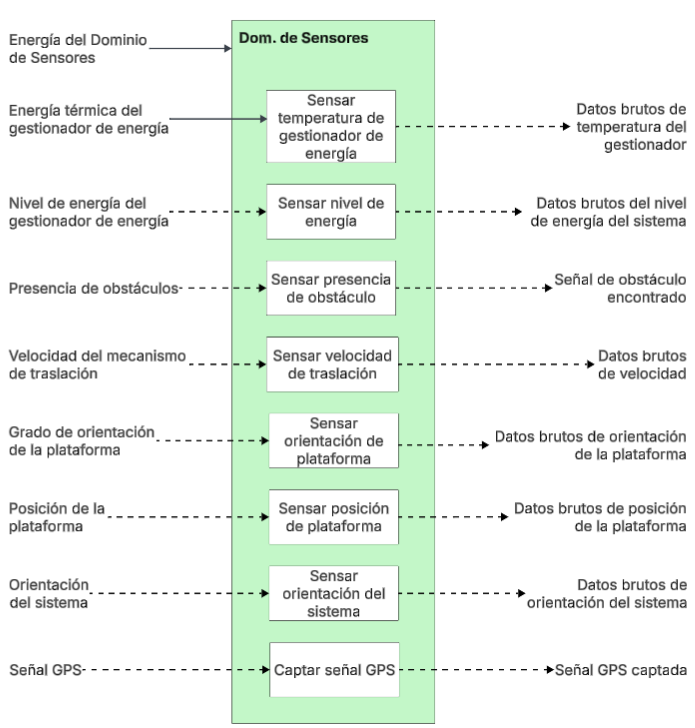
\includegraphics[width=0.8\textwidth]{Imagenes/A3_DominioSensores.png} \par\medskip
	
	\raggedright
	\footnotesize \textit{Nota.} Elaboración propia.
	\label{fig:Avance3_DomSensores}
\end{figure}
\subsection{Dominio de Control}

El Dominio de Control opera como el núcleo lógico y computacional del sistema, encargado de procesar la información recibida, gestionar la seguridad energética, registrar los datos climáticos y comandar tanto la navegación como los actuadores. Todo el subsistema es alimentado por la energía del Dominio de Control y el Dominio de Comunicaciones. Está compuesto de las siguientes funciones:

\begin{enumerate}
	\item \textbf{Procesar datos meteorológicos:} Recibe los datos meteorológicos brutos, enviándolos hacia el exterior como datos meteorológicos procesados y transfiriéndolos simultáneamente al bloque de registro.
	\item \textbf{Registrar datos meteorológicos:} Escribe la información recibida generando el flujo de comunicación con memoria externa de salida para el respaldo físico de los datos.
	\item \textbf{Procesar temperatura de gestionador:} Interpreta los datos brutos de temperatura del gestionador provenientes del módulo de energía.
	\item \textbf{Procesar nivel de energía:} Interpreta los datos brutos del nivel de energía del sistema y emite directamente la información sobre estado de energía hacia el exterior.
	\item \textbf{Procesar estado de energía del sistema:} Recibe y hace converger los flujos lógicos internos de temperatura y nivel de energía procesados para devolver una variable de estado general.
	\item \textbf{Controlar estado de energía del sistema:} Evalúa la variable del bloque anterior para generar la señal de control del estado de energía del sistema, la cual interactúa con el interruptor de encendido.
	\item \textbf{Procesar rutas de inspección:} Extrae la información espacial ingresada desde la comunicación con memoria externa de entrada para generar internamente la información procesada de rutas de inspección.
	\item \textbf{Procesar posición del sistema:} Interpreta los datos de posición del sistema brutos externos para derivar las coordenadas de posición del sistema.
	\item \textbf{Procesar presencia de obstáculo:} Evalúa la señal de obstáculo encontrado proveniente de los sensores, retransmitiéndola de forma directa como salida de alerta y generando internamente la posición de obstáculo.
	\item \textbf{Procesar orientación del sistema:} Recibe e interpreta los datos brutos de orientación del sistema para alimentar los cálculos de navegación espacial.
	\item \textbf{Procesar velocidad de traslación, procesar orientación de la plataforma y procesar posición de la plataforma:} Son tres funciones paralelas que interpretan de forma independiente los datos brutos de velocidad, los datos brutos de orientación de la plataforma y los datos brutos de posición de la plataforma, provenientes de la retroalimentación de los mecanismos físicos.
	\item \textbf{Controlar movimiento de actuador de traslación, orientación de plataforma y posicionamiento de plataforma):} Constituyen las tres etapas finales de salida de este dominio. Integran de forma conjunta las variables de navegación (rutas, coordenadas, orientación del sistema y obstáculos) con sus respectivos lazos de retroalimentación para emitir las señales de control respectivas.
\end{enumerate}

\begin{figure}[H]
	\captionsetup{justification=raggedright, singlelinecheck=false, labelsep=none}
	
	\caption[Dominio de control de la estructura de funciones.]{} 
	
	\textit{Dominio de control de la estructura de funciones.} \par\medskip
	
	\makebox[\textwidth][c]{ 
		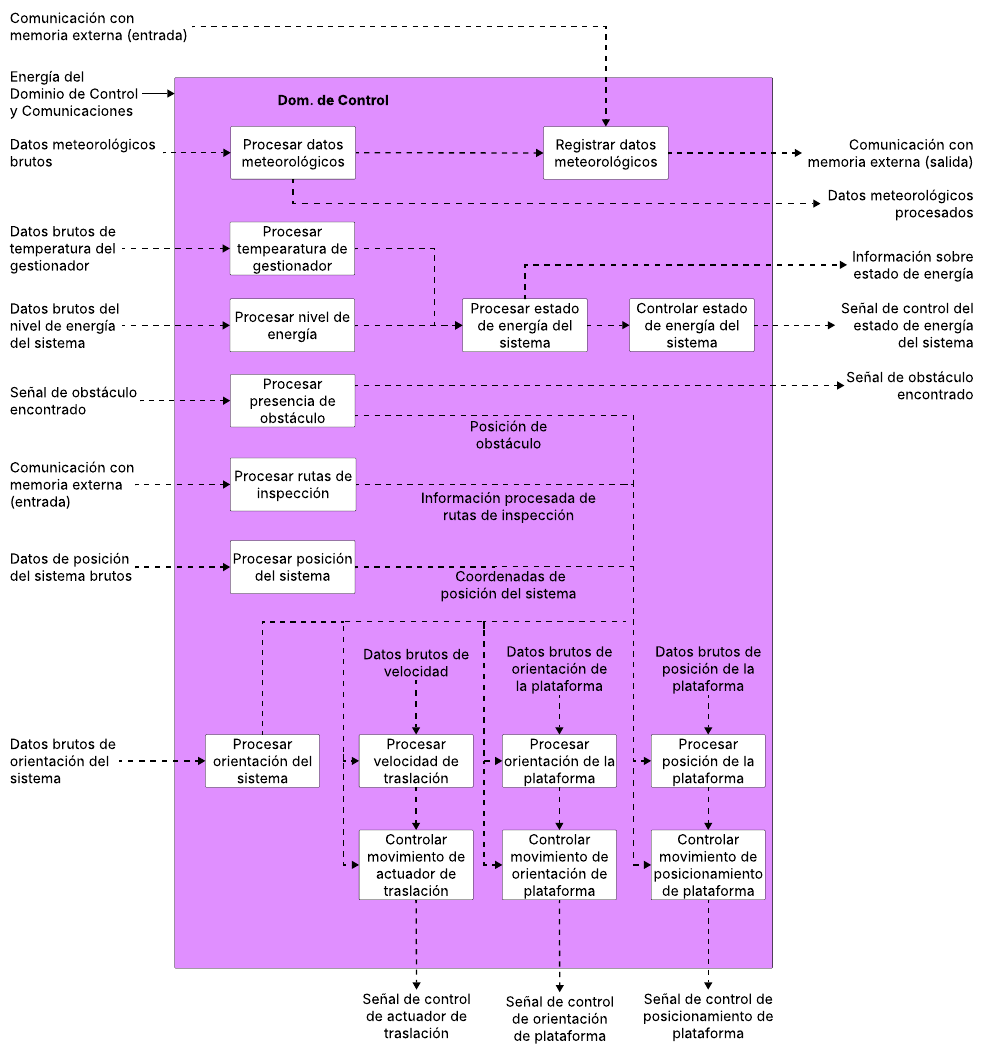
\includegraphics[width=0.9\textwidth]{Imagenes/A3_DominioControl.png}
	} \par\medskip
	
	\raggedright
	\footnotesize \textit{Nota.} Elaboración propia.
	\label{fig:Avance3_DomControl}
\end{figure}

\subsection{Dominio de Comunicación}

El Dominio de Comunicación actúa como el puente de telemetría entre el robot y la red externa del parque fotovoltaico. Para su operatividad, todo este subsistema se encuentra alimentado por el flujo de energía del Dominio de Control y el Dominio de Comunicaciones. El dominio se compone de las siguientes funciones:

\begin{enumerate}
	\item \textbf{Procesar señal GPS recibida:} Capta e interpreta la señal de radiofrecuencia satelital proveniente del entorno para transformarla y entregar los datos de posición del sistema brutos, los cuales son requeridos por la lógica de navegación interna.
	
	\item \textbf{Procesar señal de mando recibida:} Gestiona el enlace interactivo de entrada proveniente de la señal de control de telecomunicación. Principalmente, esta función decodifica la trama de los comandos de telemetría, asegurando una respuesta inmediata del robot frente a instrucciones del usuario.
	
	\item \textbf{Transmitir estado telemétrico:} Emite la señal de estado de transmisión telemétrica hacia el exterior, lo que permite a la estación base monitorear de forma continua la calidad, latencia e integridad del enlace de red con el vehículo.
	
	\item \textbf{Transmitir datos meteorológicos:} Constituye la etapa final del reporte climático y operativo. Esta función recibe los datos meteorológicos procesados desde el dominio de control, y seguidamente codifica y empaqueta la información en un payload para enviarla hacia la estación base en forma de paquetes de datos meteorológicos consolidados.
\end{enumerate}

\begin{figure}[H]
	\captionsetup{justification=raggedright, singlelinecheck=false, labelsep=none}
	
	\caption[Dominio de comunicaciones de la estructura de funciones.]{} 
	
	\textit{Dominio de comunicaciones de la estructura de funciones.} \par\medskip
	
	\makebox[\textwidth][c]{ 
		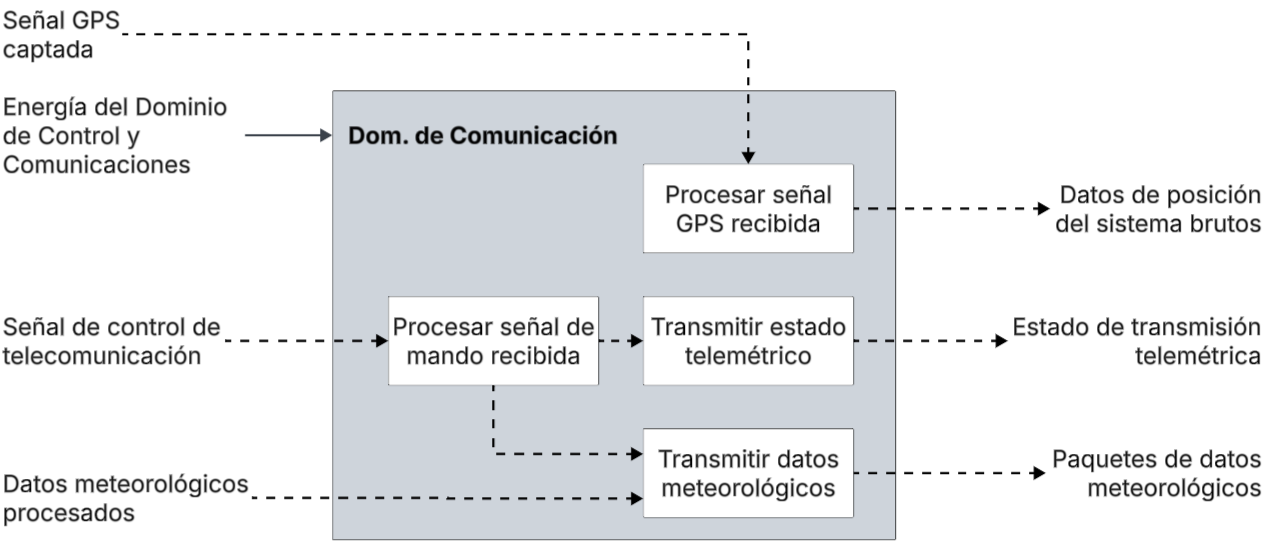
\includegraphics[width=0.8\textwidth]{Imagenes/A3_DominioComunicacion.png}
	} \par\medskip
	
	\raggedright
	\footnotesize \textit{Nota.} Elaboración propia.
	\label{fig:Avance3_DomComunicacion}
\end{figure}

\subsection{Dominio de Interfaz}

El Dominio de Interfaz, mostrado en la \ref{
Avance3_Interfaz} desempeña un rol dual en la arquitectura del robot: por un lado, actúa como el puerto de conexión para la instrumentación climática periférica y, por otro, se encarga de exteriorizar los estados operativos y advertencias críticas hacia el personal en el parque fotovoltaico. Para su funcionamiento general, todos los componentes de este subsistema son alimentados directamente por el flujo de energía del Dominio de Interfaz. El dominio cuenta con los siguientes bloques de función:

\begin{enumerate}
	\item \textbf{Accionar movimiento de traslación:} Recibe la señal de control del actuador de traslación y la transforma en la energía cinética necesaria para ejecutar el desplazamiento principal del robot.
	\item \textbf{Accionar movimiento de orientación de plataforma:} Procesa la señal de control de orientación y genera la energía cinética correspondiente para ajustar este parámetro en la plataforma de medición.
	\item \textbf{Accionar movimiento de posicionamiento de plataforma:} Recibe la señal de control de posicionamiento y la convierte en la energía cinética requerida para el ajuste físico final de la plataforma.
\end{enumerate}

\begin{figure}[H]
	\captionsetup{justification=raggedright, singlelinecheck=false, labelsep=none}
	
	\caption[Dominio de interfaz de la estructura de funciones.]{} 
	
	\textit{Dominio de interfaz de la estructura de funciones.} \par\medskip
	
	\makebox[\textwidth][c]{ 
		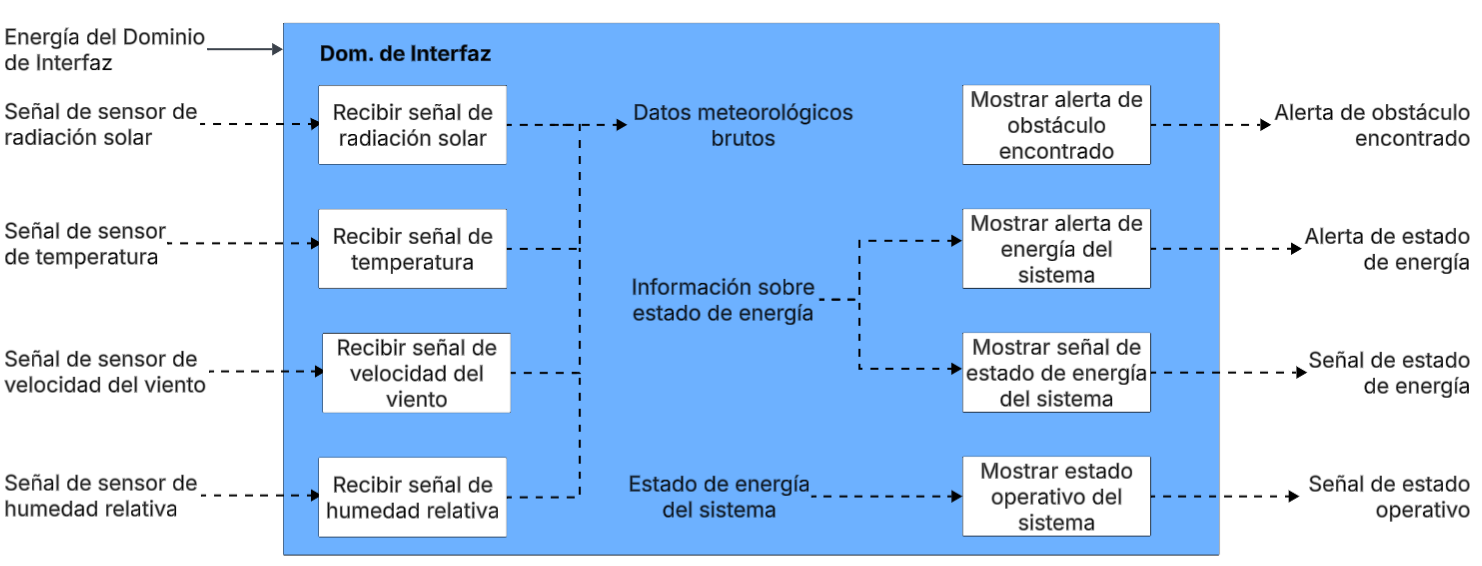
\includegraphics[width=1.0\textwidth]{Imagenes/A3_DominioInterfaz.png}
	} \par\medskip
	
	\raggedright
	\footnotesize \textit{Nota.} Elaboración propia.
	\label{fig:Avance3_DomInterfaz}
\end{figure}

\subsection{Dominio de Actuadores}
El Dominio de Actuadores es el encargado de transformar la energía eléctrica y las instrucciones lógicas en los esfuerzos cinéticos necesarios para la operación física del robot y el ajuste de sus instrumentos. Para su funcionamiento general, todo este subsistema es alimentado por el flujo de energía del Dominio de Actuadores. El dominio se compone de las siguientes funciones:

\begin{enumerate}
	\item \textbf{Accionar movimiento de traslación:} Recibe la señal de control del actuador de traslación y la transforma en la energía cinética necesaria para ejecutar el desplazamiento principal del robot.
	\item \textbf{Accionar movimiento de orientación de plataforma:} Procesa la señal de control de orientación y genera la energía cinética correspondiente para ajustar este parámetro en la plataforma de medición.
	\item \textbf{Accionar movimiento de posicionamiento de plataforma:} Recibe la señal de control de posicionamiento y la convierte en la energía cinética requerida para el ajuste físico final de la plataforma.
\end{enumerate}

\begin{figure}[H]
	\captionsetup{justification=raggedright, singlelinecheck=false, labelsep=none}
	
	\caption[Dominio de actuadores de la estructura de funciones.]{} 
	
	\textit{Dominio de actuadores de la estructura de funciones.} \par\medskip
	
	\centering
	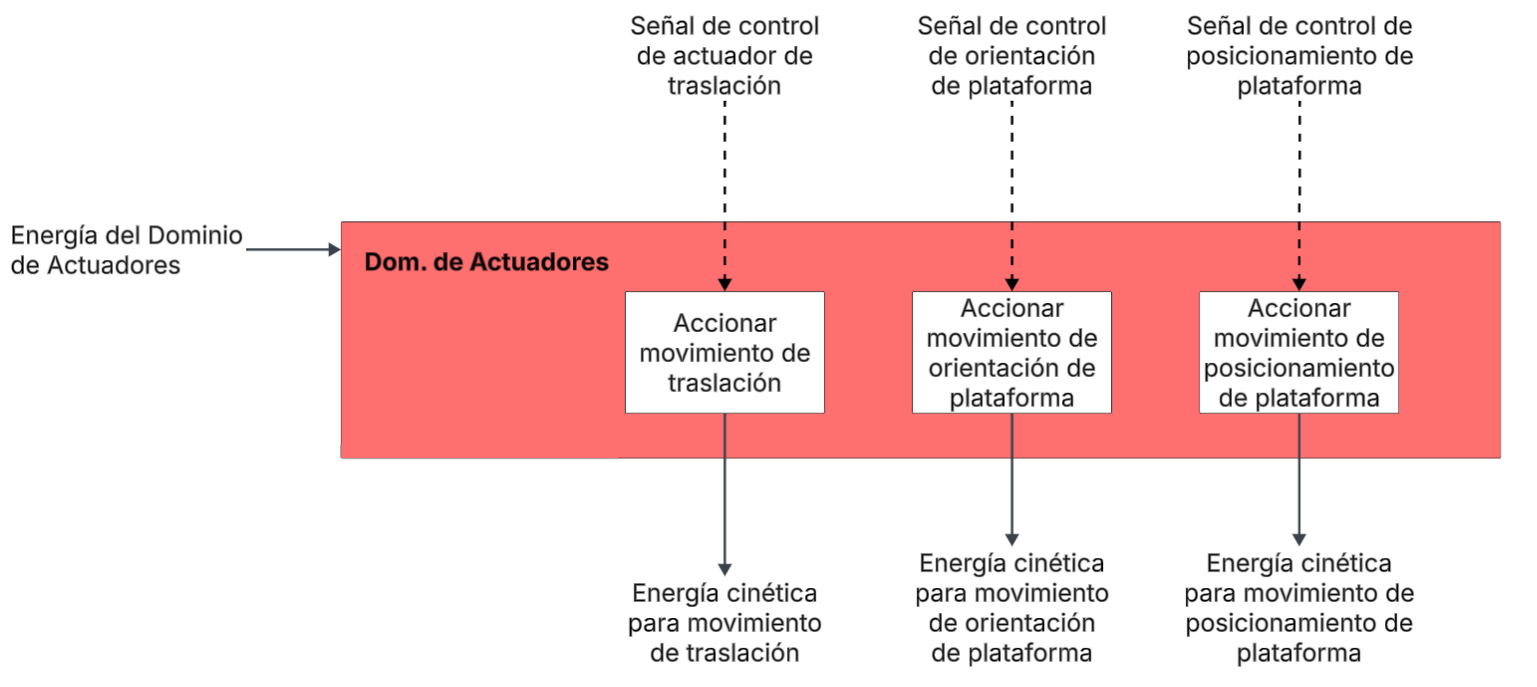
\includegraphics[width=0.99\textwidth]{Imagenes/A3_DominioActuadores.png} \par\medskip
	
	\raggedright
	\footnotesize \textit{Nota.} Elaboración propia.
	\label{fig:Avance3_DomActuadores}
\end{figure}

\subsection{Dominio Mecánico}

El Dominio Mecánico conforma el soporte estructural del vehículo y materializa las interacciones dinámicas y físicas con el entorno del parque solar. Está compuesto de las siguientes funciones:

\begin{enumerate}
	\item \textbf{Soportar plataforma de medición de radiación:} Sostiene la carga física de la instrumentación climática frente a las vibraciones mecánicas del entorno.
	\item \textbf{Proteger componentes internos:} Aísla el equipo para garantizar la integridad de la tecnología frente a factores externos como la suciedad del ambiente.
	\item \textbf{Soportar componentes:} Provee la base física unificada y el soporte estructural estático general para el resto del sistema.
	\item \textbf{Alojar gestionador de energía:} Provee la contención estructural física específica para el gestionador del sistema de energía.
	\item \textbf{Alojar memoria externa:} Actúa como la interfaz material que recibe la memoria externa física. Transmite la comunicación de entrada (rutas de inspección y formatos) al control y recibe la señal de salida para grabar los datos registrados.
	\item \textbf{Generar movimiento de traslación:} Transforma la energía cinética recibida en el desplazamiento general sobre el terreno, retroalimentando al sistema con la velocidad del mecanismo de traslación.
	\item \textbf{Orientar plataforma de medición de radiación:} Utiliza la energía cinética proveniente de los actuadores para ejecutar el cambio de ángulo, entregando como información el grado de orientación de la plataforma.
	\item \textbf{Posicionar plataforma de medición de radiación:} Emplea la energía cinética correspondiente para su ajuste espacial final, suministrando la posición de la plataforma para cerrar los lazos de control y generando las vibraciones emitidas hacia el exterior.
\end{enumerate}
\begin{figure}[H]
	\captionsetup{justification=raggedright, singlelinecheck=false, labelsep=none}
	
	\caption[Dominio mecánico de la estructura de funciones.]{} 
	
	\textit{Dominio mecánico de la estructura de funciones.} \par\medskip
	
	\makebox[\textwidth][c]{ 
		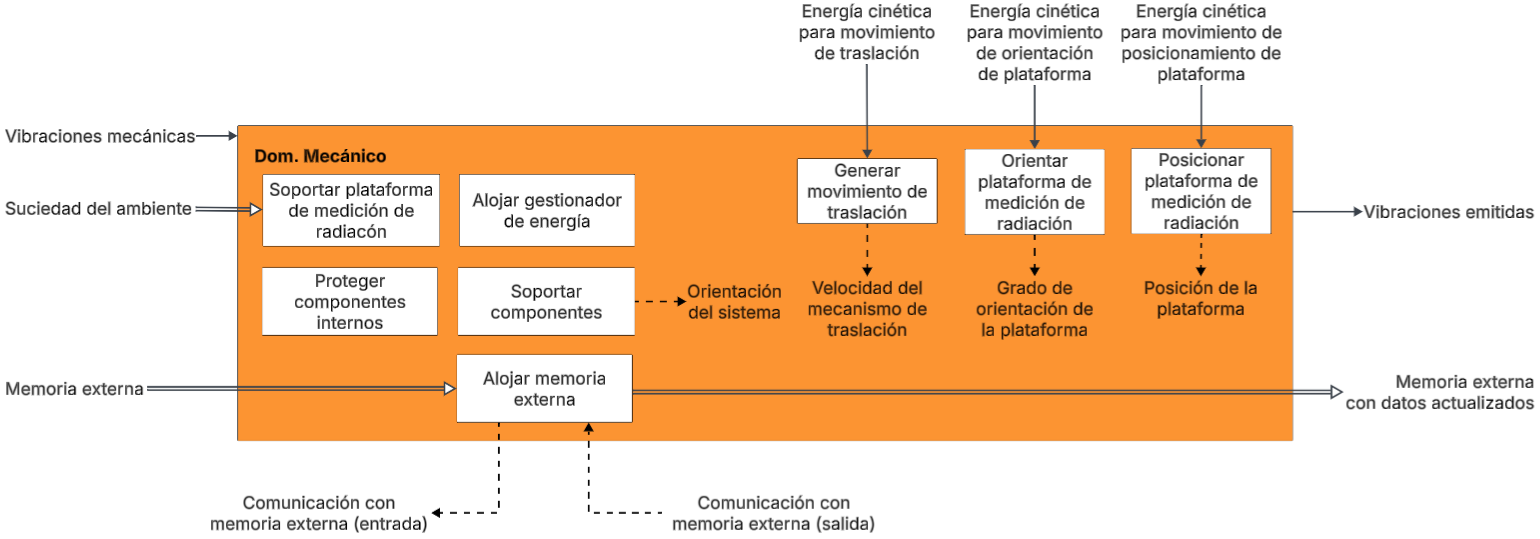
\includegraphics[width=1.25\textwidth]{Imagenes/A3_DominioMecanico.png}
	} \par\medskip
	
	\raggedright
	\footnotesize \textit{Nota.} Elaboración propia.
	\label{fig:Avance3_DomMecanico}
\end{figure}

\section{Matriz Morfológica}

Una vez completada la abstracción del sistema en la Estructura de Funciones, se procede con la búsqueda sistemática de principios de solución clasificados en la Matriz Morfológica, que permite desglosar las funciones elementales y proponer para cada una de distintos portadores de función o alternativas tecnológicas. El objetivo de esta sección es establecer un abanico amplio de principios físicos, mecánicos, electrónicos y de software que sean capaces de resolver las tareas del robot, para posteriormente combinarlos y generar los conceptos de solución integrales.
% --- Dominio de Energía ---
\begin{center}
	\footnotesize
	\begin{xltabular}{\textwidth}{|p{3.5cm}|>{\centering\arraybackslash}X|>{\centering\arraybackslash}X|>{\centering\arraybackslash}X|}
		\caption{Matriz Morfológica del Dominio de Energía.}
		\label{tab:matriz_energia} \\
		\hline
		\rowcolor[HTML]{D9E1F2} 
		\textbf{Función Parcial} & \textbf{Solución 1} & \textbf{Solución 2} & \textbf{Solución 3} \\ \hline
		\endfirsthead
		
		\multicolumn{4}{c}%
		{{\bfseries \tablename\ \thetable{} -- Continuación de la página anterior}} \\
		\hline
		\rowcolor[HTML]{D9E1F2} 
		\textbf{Función Parcial} & \textbf{Solución 1} & \textbf{Solución 2} & \textbf{Solución 3} \\ \hline
		\endhead
		
		\hline
		\endfoot
		
		\hline
		\endlastfoot
		
		\textbf{1. Recibir energía eléctrica} & 
		Conector Plug Jack DC \par\smallskip 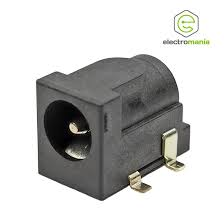
\includegraphics[width=0.7\linewidth]{ImagenesMatriz/ConectorPlugJackDC.jpg} & 
		Conector de alta corriente XT60 \par\smallskip 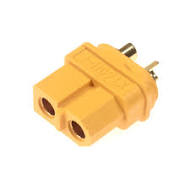
\includegraphics[width=0.7\linewidth]{ImagenesMatriz/ConectorAltaCorriente.jpg} & 
		Contactos magnéticos \par\smallskip 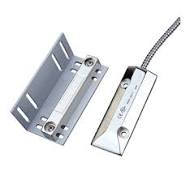
\includegraphics[width=0.7\linewidth]{ImagenesMatriz/ConectorContactoMagnetico.jpg} \\ \hline
		
		\textbf{2. Proteger sistema eléctrico} & 
		Fusible cerámico de cartucho \par\smallskip 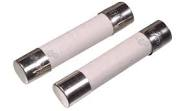
\includegraphics[width=0.7\linewidth]{ImagenesMatriz/FusibleCeramico.jpg} & 
		Fusible electrónico eFuse \par\smallskip 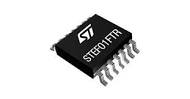
\includegraphics[width=0.9\linewidth]{ImagenesMatriz/eFuse.jpg} & 
		Disyuntor termomagnético \par\smallskip 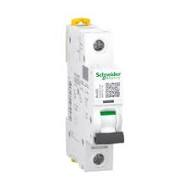
\includegraphics[width=0.7\linewidth]{ImagenesMatriz/DisyuntorTermomagnetico.jpg} \\ \hline
		
		\textbf{3. Gestionar energía eléctrica} & 
		Batería NiMH + Battery Management System \par\smallskip 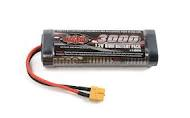
\includegraphics[width=0.7\linewidth]{ImagenesMatriz/NiMh.jpg} & 
		Batería LiIon + Battery Management System \par\smallskip 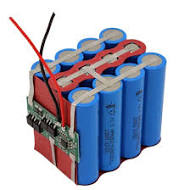
\includegraphics[width=0.7\linewidth]{ImagenesMatriz/LiIon.jpg} & 
		Batería LiPO + Battery Management System \par\smallskip 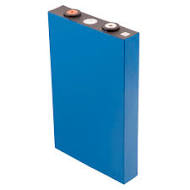
\includegraphics[width=0.7\linewidth]{ImagenesMatriz/LiPo.jpg} \\ \hline
		
		\textbf{4. Activar energía eléctrica} & 
		Seccionador rotativo manual \par\smallskip 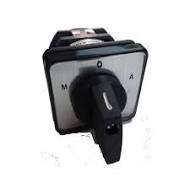
\includegraphics[width=0.7\linewidth]{ImagenesMatriz/Rotativo.jpg} & 
		Relé de estado sólido \par\smallskip 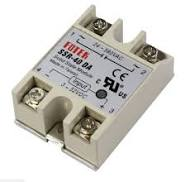
\includegraphics[width=0.7\linewidth]{ImagenesMatriz/ReleEstadoSolido.jpg} & 
		Contactor mecánico \par\smallskip 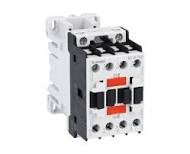
\includegraphics[width=0.7\linewidth]{ImagenesMatriz/Contactor.jpg} \\ \hline
		
		\textbf{5. Regular energía de Interfaz} \vspace{0.2cm} & 
		\multirow{3}{=}{\centering Regulador de bomba de carga fija\par\vspace{0.2cm} 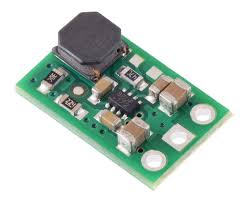
\includegraphics[width=0.65\linewidth]{ImagenesMatriz/PumpChargeRegulador.jpg}} & 
		\multirow{3}{=}{\centering Regulador lineal LDO \par\vspace{0.2cm} 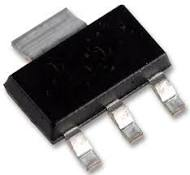
\includegraphics[width=0.65\linewidth]{ImagenesMatriz/ReguladorLDO.jpg}} & 
		\multirow{3}{=}{\centering Regulador Shunt \par\vspace{0.2cm} 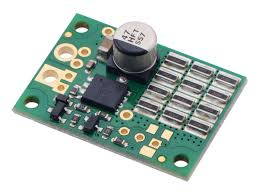
\includegraphics[width=0.65\linewidth]{ImagenesMatriz/ShuntRegulator.jpg}} \\ \cline{1-1}
		
		\textbf{6. Regular energía de Control/Comunicación} \vspace{0.2cm} & & & \\ \cline{1-1}
		
		\textbf{7. Regular energía de Sensores} \vspace{0.6cm} & & & \\ \hline
		%
		\textbf{8. Regular energía de Actuadores} & 
		Convertidor Buck DC-DC \par\smallskip 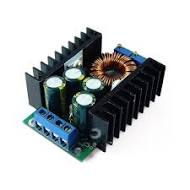
\includegraphics[width=0.7\linewidth]{ImagenesMatriz/ConvertidorBuck.jpg} & 
		Regulador de bomba de carga \par\smallskip 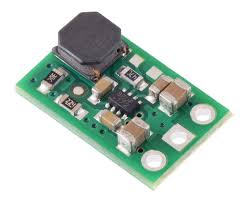
\includegraphics[width=0.7\linewidth]{ImagenesMatriz/PumpChargeRegulador.jpg} & 
		Regulador lineal LDO \par\smallskip 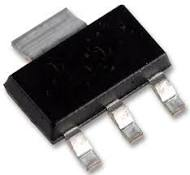
\includegraphics[width=0.7\linewidth]{ImagenesMatriz/ReguladorLDO.jpg} \\ \hline
		%
		\pagebreak
		
		% --- INICIO BLOQUE 5-8 ---
		\textbf{9. Energizar Interfaz} \vspace{0.6cm} & 
		\multirow{3}{=}{\centering Cable trenzado estándar \par\vspace{0.2cm} 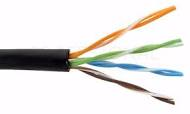
\includegraphics[width=0.65\linewidth]{ImagenesMatriz/CableTrenzado.jpg}} & 
		\multirow{3}{=}{\centering Conectores circular roscado \par\vspace{0.2cm} 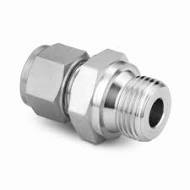
\includegraphics[width=0.65\linewidth]{ImagenesMatriz/ConectorRoscado.jpg}} & 
		\multirow{3}{=}{\centering Barras colectoras Busbars \par\vspace{0.2cm} 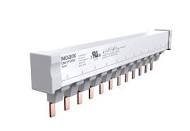
\includegraphics[width=0.65\linewidth]{ImagenesMatriz/Busbar.jpg}} \\ \cline{1-1}
		
		\textbf{10. Energizar Control/Comm.} \vspace{0.6cm} & & & \\ \cline{1-1}
		
		\textbf{11. Energizar Sensores} \vspace{0.6cm} & & & \\ \hline
		% --- FIN BLOQUE 9-11 ---
		
		\textbf{12. Energizar Actuadores} & 
		Cable de Baja Tensión \par\smallskip 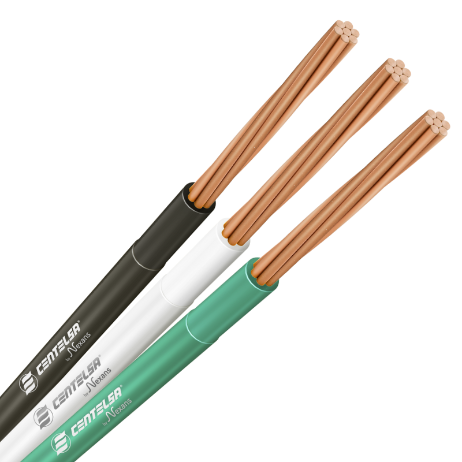
\includegraphics[width=0.7\linewidth]{ImagenesMatriz/CableBajaTension.png} & 
		Conector Circular Roscado \par\smallskip 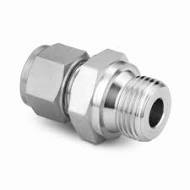
\includegraphics[width=0.7\linewidth]{ImagenesMatriz/ConectorRoscado.jpg} & 
		Barras colectoras Busbars \par\smallskip 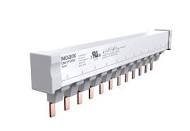
\includegraphics[width=0.7\linewidth]{ImagenesMatriz/Busbar.jpg} \\ \hline
		%%
		\textbf{13. Regular energía eléctrica de sensores meteorológicos} & 
		Regulador de bomba de carga \par\smallskip 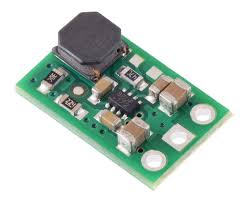
\includegraphics[width=0.7\linewidth]{ImagenesMatriz/PumpChargeRegulador.jpg} & 
		Regulador lineal LDO \par\smallskip 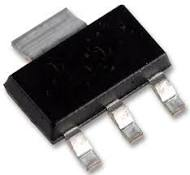
\includegraphics[width=0.7\linewidth]{ImagenesMatriz/ReguladorLDO.jpg} & 
		Regulador Shunt \par\smallskip 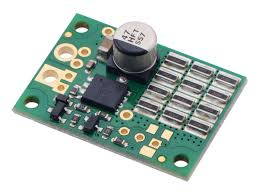
\includegraphics[width=0.7\linewidth]{ImagenesMatriz/ShuntRegulator.jpg} \\ \hline
		%%
		\textbf{14. Energizar  sensores meteorológicos} & 
		Cable trenzado estándar \par\smallskip 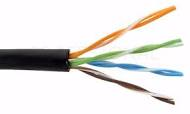
\includegraphics[width=0.7\linewidth]{ImagenesMatriz/CableTrenzado.jpg} & 
		Conector circular roscado \par\smallskip 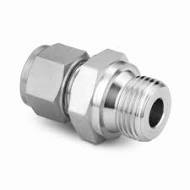
\includegraphics[width=0.7\linewidth]{ImagenesMatriz/ConectorRoscado.jpg} & 
		Barras colectoras Busbars \par\smallskip 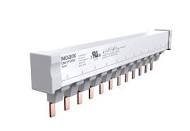
\includegraphics[width=0.7\linewidth]{ImagenesMatriz/Busbar.jpg} \\ \hline
		
	\end{xltabular}
\end{center}

\begin{itemize}
	\item \textbf{Recibir energía eléctrica:} para esta función se evaluó el conector Plug Jack DC, que permite una conexión lineal simple para corrientes medias; el conector de alta corriente XT60, el cual asegura una conexión física firme capaz de soportar las altas corrientes requeridas para la carga de baterías; y los contactos magnéticos, que facilitan un acople automático con la estación de carga sin requerir movimientos de gran exactitud por parte del vehículo.
	
	\item \textbf{Proteger sistema eléctrico:} se analizó el fusible electrónico eFuse por su corte rápido y posibilidad de restablecimiento automático, ideal para sistemas autónomos; el disyuntor termomagnético, que ofrece una protección robusta ante cortocircuitos pero exige rearme manual; y el fusible cerámico de cartucho, una opción de bajo costo y alta capacidad de ruptura que requiere reemplazo físico tras activarse.
	
	\item \textbf{Gestionar energía eléctrica:} las opciones contemplan la batería LiPO con Battery Management System (BMS), destacada por sus altas tasas de descarga y bajo peso; la batería LiIon con BMS, que proporciona una alta densidad energética y larga vida útil para asegurar la autonomía de operación del robot; y la batería NiMH con BMS, una alternativa estable frente a riesgos térmicos pero con la desventaja de tener un mayor peso y menor densidad de energía.
	
	\item \textbf{Activar energía eléctrica:} se consideró el relé de estado sólido, que permite la conmutación mediante señales de control sin partes móviles; el contactor mecánico, útil para manejar los picos de corriente durante el arranque de los motores; y el seccionador rotativo manual, que actúa como un elemento de corte físico directo para asegurar la desconexión total.
	
	\item \textbf{Regular energía Interfaz, Regular energía Control/Comm, Regular energía Sensores y Regular energía eléctrica de sensores meteorológicos:} se evaluó el regulador Shunt, de diseño simple pero térmicamente ineficiente al disipar el exceso de energía como calor; el regulador lineal LDO, que ofrece un voltaje de salida estable y con bajo ruido eléctrico, indispensable para los microcontroladores y la instrumentación; y el regulador de bomba de carga, útil para elevar o reducir voltajes en espacios reducidos pero limitado a bajas corrientes.
	
	\item \textbf{Regular energía de Actuadores:} para esta etapa de regulación de potencia se analizó el regulador lineal LDO, que entrega un voltaje limpio pero genera demasiada pérdida térmica frente a la demanda de los motores; el regulador de bomba de carga, de circuito compacto pero con capacidad de corriente insuficiente; y el convertidor Buck DC-DC, que posee una alta eficiencia de conversión energética para soportar el consumo dinámico de los mecanismos mecánicos.
	
	\item \textbf{Energizar Interfaz, Energizar Control/Comm., Energizar Sensores y Energizar sensores meteorológicos:} se propusieron las barras colectoras para facilitar una distribución rígida de alimentación entre componentes fijos; el cable trenzado estándar, que aporta flexibilidad para el ruteo interno en la caja de control; y la combinación de conectores circulares roscados con barras colectoras, que garantiza una conexión firme y resistente a las desconexiones causadas por las vibraciones del terreno.
	
	\item \textbf{Energizar Actuadores (Distribución):} se consideraron los contactos magnéticos, de acople rápido pero vulnerables a perder continuidad por los impactos del movimiento; el cable trenzado estándar, que proporciona la tolerancia mecánica necesaria para llevar la energía hasta los ejes móviles de los actuadores; y las barras colectoras Busbars, que soportan altas corrientes de manera eficiente y robusta.
\end{itemize}


\subsection{Dominio de Sensores}


\begin{center}
	\footnotesize
	\begin{xltabular}{\textwidth}{|p{3.5cm}|>{\centering\arraybackslash}X|>{\centering\arraybackslash}X|>{\centering\arraybackslash}X|}
		\caption{Matriz Morfológica del Dominio de Sensores.}
		\label{tab:matriz_sensores} \\
		\hline
		\rowcolor[HTML]{D9E1F2} 
		\textbf{Función Parcial} & \textbf{Solución 1} & \textbf{Solución 2} & \textbf{Solución 3} \\ \hline
		\endfirsthead
		
		\multicolumn{4}{c}%
		{{\bfseries \tablename\ \thetable{} -- Continuación de la página anterior}} \\
		\hline
		\rowcolor[HTML]{D9E1F2} 
		\textbf{Función Parcial} & \textbf{Solución 1} & \textbf{Solución 2} & \textbf{Solución 3} \\ \hline
		\endhead
		
		\hline
		\endfoot
		
		\hline
		\endlastfoot
		
		\textbf{1. Sensar temperatura del gestionador} & 
		Termistor NTC \par\smallskip 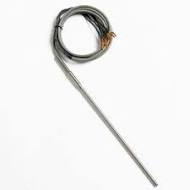
\includegraphics[width=0.7\linewidth]{ImagenesMatriz/TermistorNTC.jpg} & 
		Termopar tipo K \par\smallskip 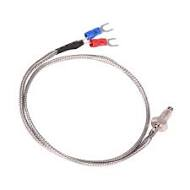
\includegraphics[width=0.7\linewidth]{ImagenesMatriz/Termopar.jpg} & 
		Sensor RTD PT100 \par\smallskip 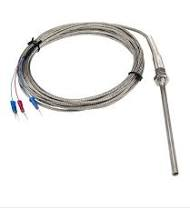
\includegraphics[width=0.7\linewidth]{ImagenesMatriz/SensorRTD.jpg} \\ \hline
		
		\textbf{2. Sensar nivel de energía del gestionador} & 
		Detector de umbral de voltaje \par\smallskip 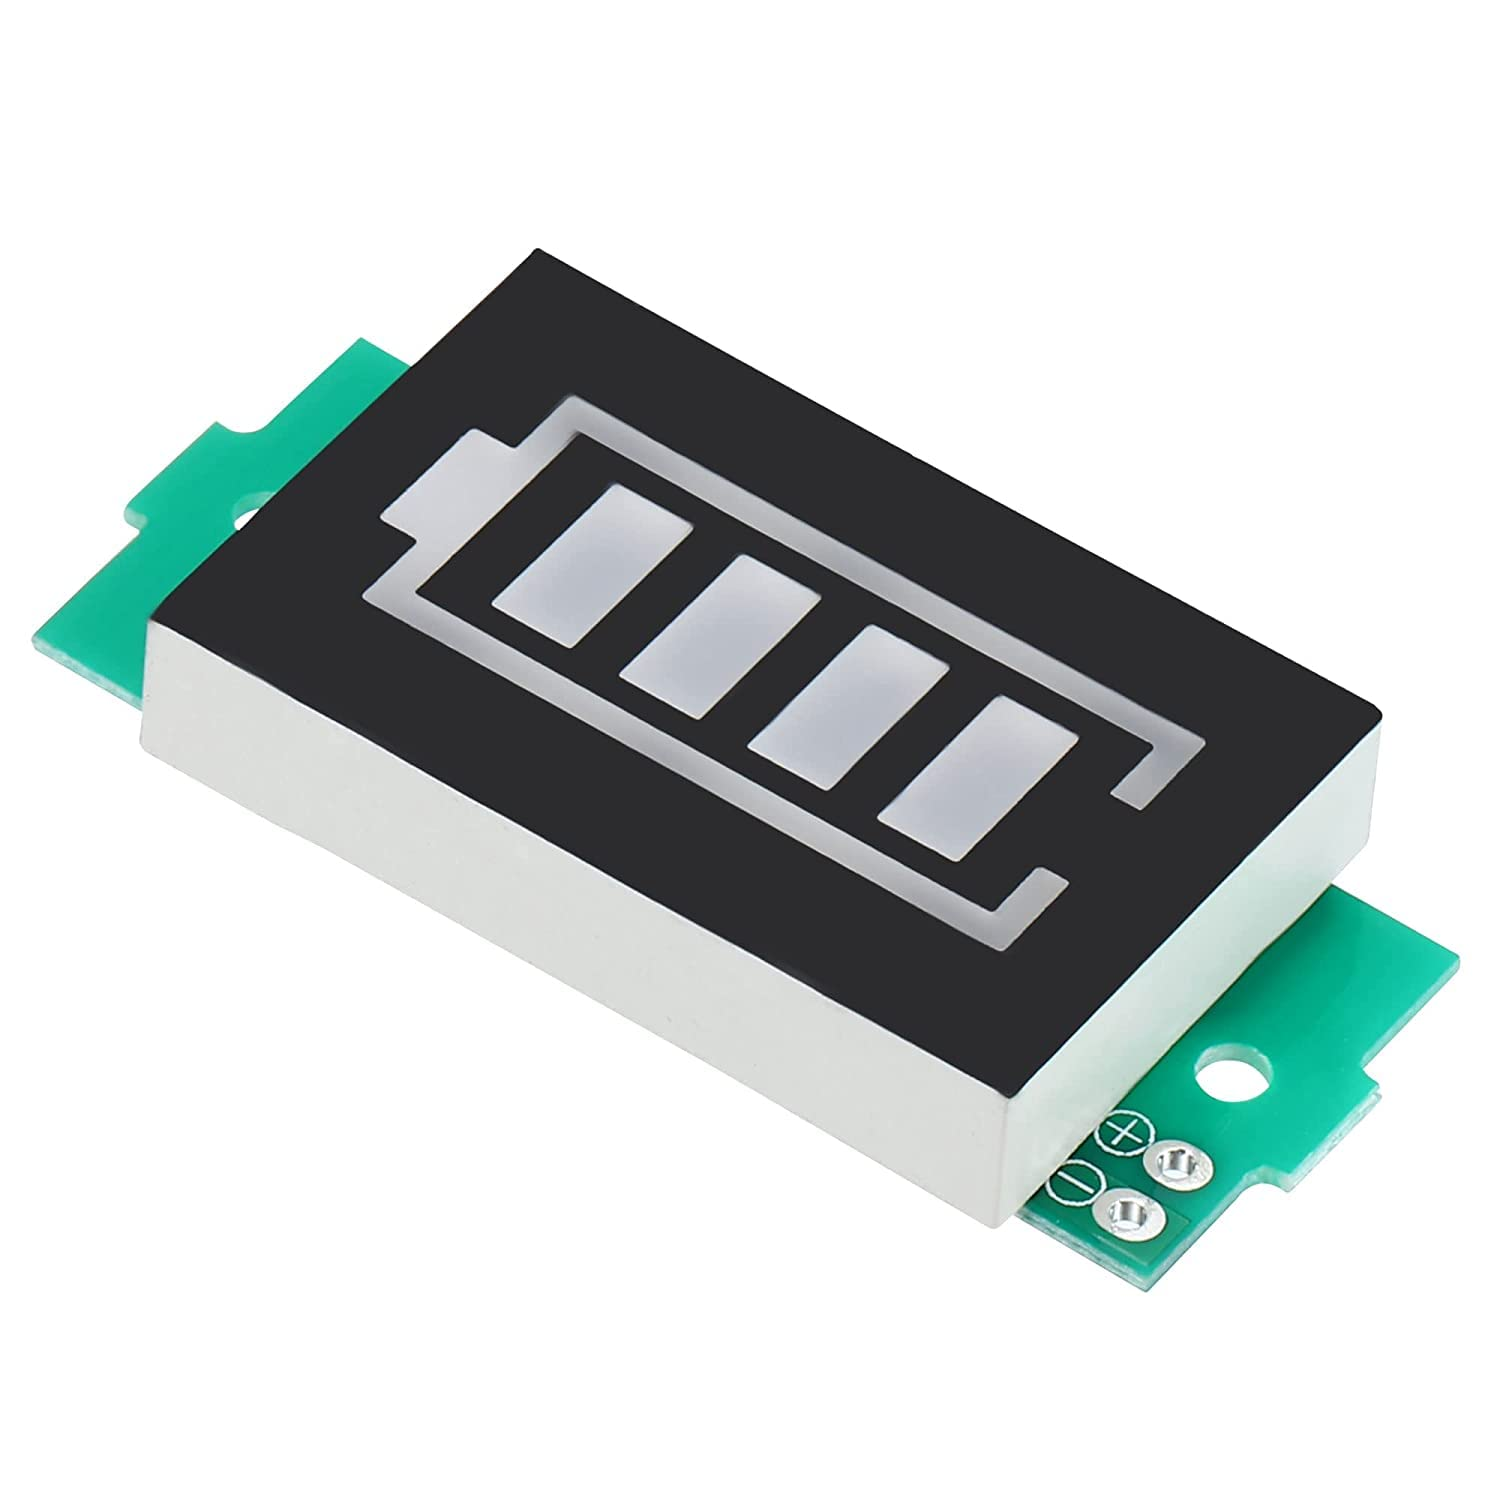
\includegraphics[width=0.7\linewidth]{ImagenesMatriz/SensorNivelVoltaje.jpg}& 
		Sensor contador de Culombios \par\smallskip 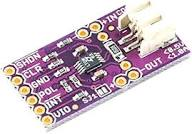
\includegraphics[width=0.7\linewidth]{ImagenesMatriz/SensorNivelCoulomb.jpg} & 
		Sensor de impedancia interna \par\smallskip 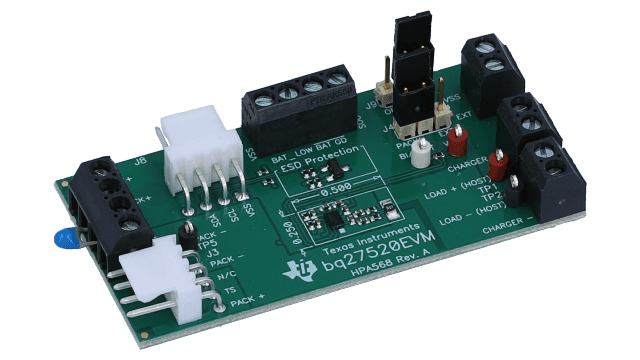
\includegraphics[width=0.9\linewidth]{ImagenesMatriz/SensorNivelImpedencia.png} \\ \hline
		
		\textbf{3. Sensar presencia de obstáculo} & 
		Sensor 3D de tiempo de vuelo \par\smallskip 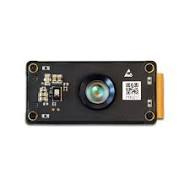
\includegraphics[width=0.7\linewidth]{ImagenesMatriz/SensorToF.jpg}& 
		Módulo CMOS \par\smallskip 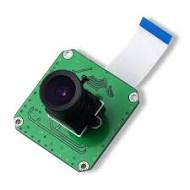
\includegraphics[width=0.7\linewidth]{ImagenesMatriz/CMOSModule.jpg} & 
		Sensor LiDAR 3D \par\smallskip 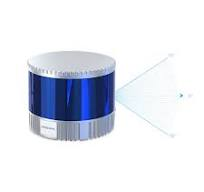
\includegraphics[width=0.9\linewidth]{ImagenesMatriz/LIDAR3D.jpg} \\ \hline
		
		\textbf{4. Sensar velocidad de traslación} & 
		Encoder rotativo incremental\par\smallskip 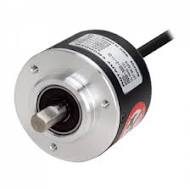
\includegraphics[width=0.7\linewidth]{ImagenesMatriz/EncoderRotativoIncremental.jpg} & 
		Unidad IMU de 9 ejes \par\smallskip 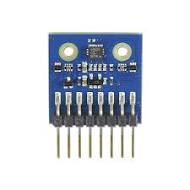
\includegraphics[width=0.7\linewidth]{ImagenesMatriz/IMU9Ejes.jpg} & 
		Radar de onda continua \par\smallskip 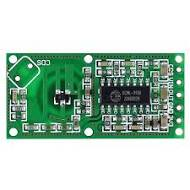
\includegraphics[width=0.7\linewidth]{ImagenesMatriz/RadarOndaContinua.jpg} \\ \hline
		
		\textbf{5. Sensar orientación plataforma} & 
		Sensor de distancia por tiempo de vuelo \par\smallskip 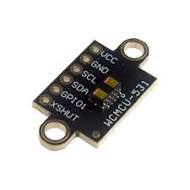
\includegraphics[width=0.7\linewidth]{ImagenesMatriz/SensorDistanciaToF.jpg} & 
		Unidad IMU de 9 ejes \par\smallskip 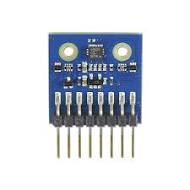
\includegraphics[width=0.7\linewidth]{ImagenesMatriz/IMU9Ejes.jpg} & 
		Encoder rotativo absoluto \par\smallskip 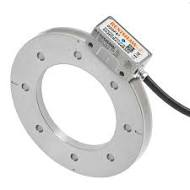
\includegraphics[width=0.7\linewidth]{ImagenesMatriz/EncoderRotativoAbsoluto.jpg} \\ \hline
		
		\textbf{6. Sensar posición de plataforma} & 
		Sensor de fin de carrera \par\smallskip 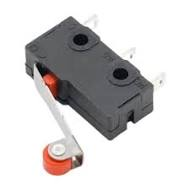
\includegraphics[width=0.7\linewidth]{ImagenesMatriz/FinDeCarrera.jpg} & 
		Potenciómetro lineal \par\bigskip 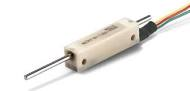
\includegraphics[width=0.7\linewidth]{ImagenesMatriz/PotenciometroLineal.jpg}& 
		Sensor de ultrasonido \par\smallskip 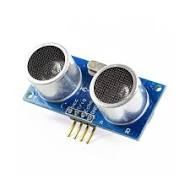
\includegraphics[width=0.7\linewidth]{ImagenesMatriz/SensorUltrasonido.jpg} \\ \hline
		
		\textbf{7. Captar señal GPS} & 
		Antena de circuito flexible \par\smallskip 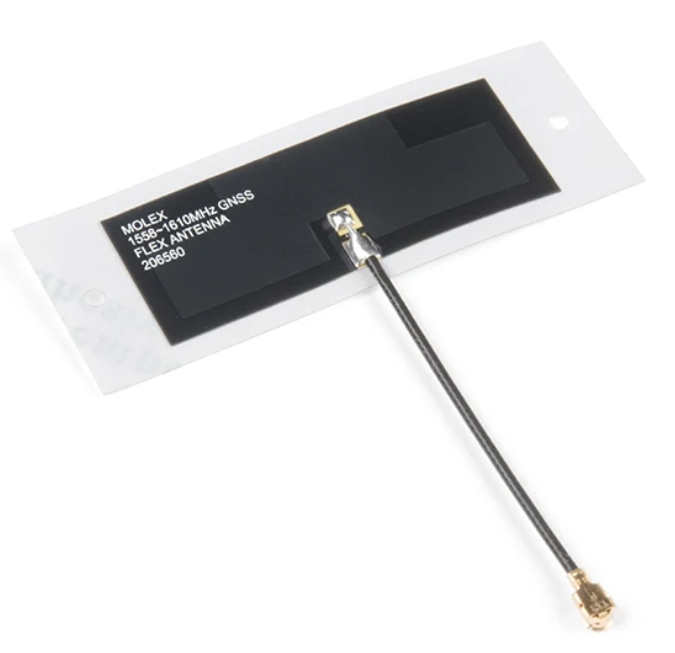
\includegraphics[width=0.7\linewidth]{ImagenesMatriz/AntenaFlexible.png} & 
		Antena de parche cerámico \par\smallskip 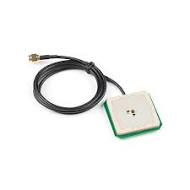
\includegraphics[width=0.7\linewidth]{ImagenesMatriz/AntenaGNSS.jpg} & 
		Antena GPS RTK \par\smallskip 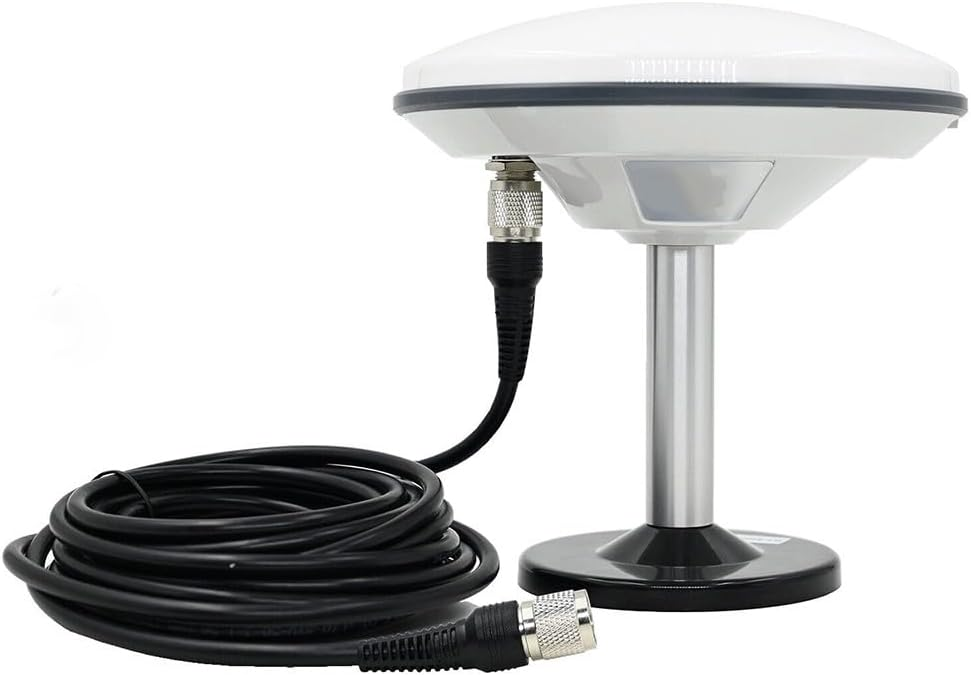
\includegraphics[width=0.7\linewidth]{ImagenesMatriz/AntenaGPSRTK.jpg} \\ \hline
		
		\textbf{8. Sensar orientación del sistema} & 
		\par\smallskip Unidad IMU de 9 ejes 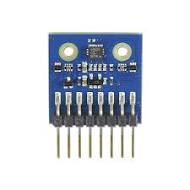
\includegraphics[width=0.7\linewidth]{ImagenesMatriz/IMU9Ejes.jpg} & 
		\par\smallskip Unidad IMU de 9 ejes  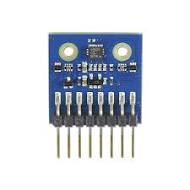
\includegraphics[width=0.7\linewidth]{ImagenesMatriz/IMU9Ejes.jpg} & 
		Matriz de sensores de distancia por tiempo de vuelo \par\smallskip 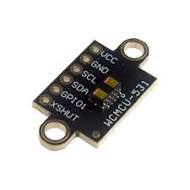
\includegraphics[width=0.7\linewidth]{ImagenesMatriz/SensorDistanciaToF.jpg} \\ \hline
		
	\end{xltabular}
\end{center}


\begin{itemize}
	\item \textbf{Sensar temperatura del gestionador:} Se evaluó el termistor NTC; el sensor RTD PT100, justificado por la necesidad de medir con precisión frente al efecto de isla de calor fotovoltaica (PVHI) y las variaciones térmicas extremas documentadas en la caracterización de microclimas \citep{Armstrong2026, Garcia2014}; y el termopar tipo K, de alta robustez mecánica.
	
	\item \textbf{Sensar nivel de energía del gestionador:} Se consideró el detector de umbral de voltaje, el cual generaría lecturas erróneas debido a las severas caídas de tensión que sufren las baterías al superar pendientes del 28\,\% \citep{GarciaSalinas2025}; el sensor de impedancia; y el contador de Culombios, principio tecnológico clave integrado en los avanzados Sistemas de Gestión de Baterías (BMS) de las estaciones meteorológicas \textit{IoT} evaluadas en el estado del arte para operar en terrenos remotos \citep{SK302020A3}.
	
	\item \textbf{Sensar presencia de obstáculo:} Se consideró el módulo \textit{CMOS}, útil para la generación de mapas espaciales \citep{CN119665962A} pero vulnerable al deslumbramiento por el albedo de los paneles; el sensor \textit{ToF} 3D; y el sensor \textit{LiDAR} 3D, tecnología indispensable extraída de los vehículos terrestres de inspección en desiertos (UGV), ya que es el único principio capaz de evadir zanjas erosivas y relieve complejo que la visión artificial simple no detecta \citep{CN221163061U, Figgis2025}.
	
	\item \textbf{Sensar velocidad de traslación:} Se analizó el \textit{encoder} rotativo incremental, el cual presentará errores críticos de odometría debido al deslizamiento de las orugas en terrenos irregulares, una limitación comprobada en los actuales vehículos de inspección solar \citep{Figgis2025}; el radar de onda continua; y la unidad \textit{IMU} de 9 ejes, requerida para la estimación inercial sin contacto con el suelo.
	
	\item \textbf{Sensar orientación (Plataforma y Sistema):} Se evaluaron el \textit{encoder} rotativo absoluto y el sensor \textit{ToF}; así como la unidad \textit{IMU} de 9 ejes. Este último es el principio técnico fundamental utilizado por las estaciones meteorológicas fotovoltaicas móviles para proveer el vector de gravedad absoluto, activar los mecanismos de nivelación \citep{CN216956405U} y asegurar la horizontalidad de la instrumentación exigida por la norma \citep{IEC61724-1_2021}.
	
	\item \textbf{Sensar posición de plataforma:} Se propuso el potenciómetro lineal; el sensor de ultrasonido, cuyo principio acústico resulta ineficiente al ser desviado por las cargas de viento extremo y las turbulencias aerodinámicas documentadas en las laderas de los parques solares \citep{Xu2024}; y el sensor de fin de carrera, seleccionado por su fiabilidad física a la intemperie.
	
	\item \textbf{Captar señal GPS:} Se evaluó la antena de parche cerámico, propensa a perder satélites al inclinarse en el relieve; la antena de circuito flexible; y la antena \textit{GPS RTK} (Real-Time Kinematic), a menudo combinada con telemetría en vehículos de inspección \citep{CN116405876A}. Su inclusión se justifica al ser la única tecnología capaz de garantizar la exactitud centimétrica indispensable para la georreferenciación de los microclimas y la corrección de ruta en la montaña \citep{Armstrong2026, Figgis2025}.
\end{itemize}


\begin{itemize}
	\item \textbf{Sensar temperatura del gestionador:} para esta función se evaluó el termistor NTC, con un bajo costo y una excelente sensibilidad para los rangos de temperatura de operación esperados en las baterías; el sensor RTD PT100, el cual brinda una alta precisión y estabilidad térmica a cambio de un mayor costo y un circuito de acondicionamiento más complejo; y el termopar tipo K, que es muy robusto y soporta rangos térmicos extremos, aunque puede presentar menor exactitud a temperatura ambiente.
	
	\item \textbf{Sensar nivel de energía del gestionador:} se consideró el sensor contador de Culombios, que permite una medición exacta del estado de carga al integrar la corriente en el tiempo; el detector de umbral de voltaje, una opción simple y económica pero cuya limitación generará lecturas falsas por las caídas de tensión al demandar alta corriente para escalar pendientes de hasta el 28\,\% \citep{GarciaSalinas2025};; y el sensor de impedancia interna, el cual es ideal para evaluar la salud y degradación de la celda a largo plazo, pero resulta complejo de implementar para mediciones continuas en operación.
	
	\item \textbf{Sensar presencia de obstáculo:} las alternativas contemplan el sensor LiDAR 3D, que otorga alta precisión y un amplio rango para el mapeo espacial, pero exige un alto costo y capacidad de procesamiento; el módulo CMOS, muy útil para la clasificación visual de los obstáculos mediante algoritmos, aunque susceptible a los deslumbramientos y reflejos propios de los paneles solares; y el sensor 3D de tiempo de vuelo, que ofrece una buena percepción de profundidad a distancias cortas y medias con una menor carga computacional.
	
	\item \textbf{Sensar velocidad de traslación:} para la retroalimentación del movimiento se analizó el encoder rotativo incremental, que proporciona una medición mecánica directa, aunque sus lecturas pueden falsearse si las ruedas deslizan; la unidad IMU de 9 ejes, que estima la velocidad sin depender de la tracción mecánica pero sufre requiere calibración y reajuste de mantenimiento; y el radar de onda continua, el cual mide la velocidad real respecto al suelo mediante el efecto Doppler, siendo totalmente inmune al deslizamiento y al polvo, aunque más costoso.
	
	\item \textbf{Sensar orientación plataforma y Sensar orientación del sistema:} se evaluó el encoder rotativo absoluto, que brinda una alta precisión para medir los ángulos articulares y retiene su posición incluso ante cortes de energía; la unidad IMU de 9 ejes, que permite obtener la orientación espacial general sin necesidad de acoples mecánicos físicos, aunque es susceptible a vibraciones e interferencias magnéticas; y el sensor de distancia por tiempo de vuelo (ToF), capaz de inferir la inclinación midiendo distancias sin contacto, pero con menor exactitud para un control rotacional estricto.
	
	\item \textbf{Sensar posición de plataforma:} se consideró el sensor de ultrasonido, una alternativa económica de medición de distancia sin contacto que, sin embargo, puede verse afectada por las corrientes de viento; el sensor de fin de carrera, que ofrece una detección de topes físicos muy robusta y simple, pero está restringida a estados discretos sin brindar una lectura continua; y el potenciómetro lineal, que entrega una retroalimentación analógica continua de la posición física, aunque sus partes móviles son vulnerables al desgaste por la suciedad del entorno.
	
	\item \textbf{Captar señal GPS:} las opciones para la recepción satelital incluyen la antena de parche cerámico, que es compacta, económica y estandarizada, pero exige una orientación estrictamente cenital y un buen plano de tierra; la antena \textit{GPS RTK} (Real-Time Kinematic), a menudo combinada con telemetría en vehículos de inspección \citep{CN116405876A}, que garantiza una exactitud indispensable para el mapeo de posición del robot en topografías complejas ; y la antena de circuito flexible, que se adapta fácilmente a la geometría interna del vehículo, pero sacrifica ganancia y eficiencia general de recepción.
	
\end{itemize}
\pagebreak
\subsection{Dominio de Control}

% --- Tabla de Control (Hardware) ---
\begin{center}
	\footnotesize
	\begin{xltabular}{\textwidth}{|p{3.5cm}|>{\centering\arraybackslash}X|>{\centering\arraybackslash}X|>{\centering\arraybackslash}X|}
		\caption{Matriz Morfológica del Dominio de Control (Hardware).}
		\label{tab:matriz_control_hw} \\
		\hline
		\rowcolor[HTML]{D9E1F2} 
		\textbf{Función Parcial} & \textbf{Solución 1} & \textbf{Solución 2} & \textbf{Solución 3} \\ \hline
		\endfirsthead
		\multicolumn{4}{c}%
		{{\bfseries \tablename\ \thetable{} -- Continuación de la página anterior}} \\
		\hline
		\rowcolor[HTML]{D9E1F2} 
		\textbf{Función Parcial} & \textbf{Solución 1} & \textbf{Solución 2} & \textbf{Solución 3} \\ \hline
		\endhead
		\hline
		\endfoot
		\hline
		\endlastfoot
		% --- INICIO BLOQUE MASIVO DE 10 FILAS ---
		\textbf{1. Procesar datos meteorológicos} & 
		\multirow{13}{=}{\centering Microcontrolador \par\vspace{0.2cm} 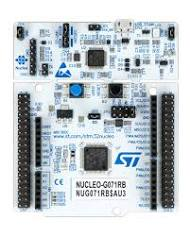
\includegraphics[width=\linewidth]{ImagenesMatriz/Microcontrolador.jpg}} & 
		\multirow{13}{=}{\centering Placa SBC \par\vspace{0.2cm} 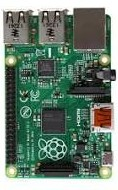
\includegraphics[width=0.7\linewidth]{ImagenesMatriz/SBC.jpg}} & 
		\multirow{13}{=}{\centering PLC \par\vspace{0.2cm} 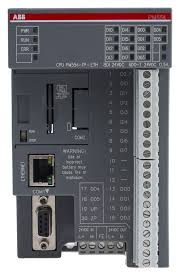
\includegraphics[width=0.7\linewidth]{ImagenesMatriz/PLC.jpg}} \\ \cline{1-1}
		\textbf{2. Procesar temperatura del gestionador} & & & \\ \cline{1-1}
		\textbf{3. Procesar nivel energía del gestionador} & & & \\ \cline{1-1}
		\textbf{4. Procesar estado energía del gestionador} & & & \\ \cline{1-1}
		\textbf{5. Procesar velocidad de traslación} & & & \\ \cline{1-1}
		\textbf{6. Procesar orientación de plataforma} & & & \\ \cline{1-1}
		\textbf{7. Procesar posición de plataforma} & & & \\ \cline{1-1}
		\textbf{8. Controlar estado energía del gestionador} & & & \\ \cline{1-1}
		\textbf{9. Controlar movimiento de traslación} & & & \\ \cline{1-1}
		\textbf{10. Controlar movimiento de orientación de plataforma} & & & \\ \cline{1-1}
		\textbf{11. Controlar posicionamiento de plataforma} & & & \\ \cline{1-1}
		\textbf{12. Controlar posicionamiento de plataforma} & & & \\ \cline{1-1} 
		\textbf{13. Procesar dirección de traslación} & & & \\ \hline
		% --- FILAS INDIVIDUALES ---
		\textbf{14. Procesar señal de obstáculo} & 
		Microcontrolador \par\smallskip 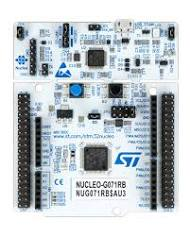
\includegraphics[width=0.7\linewidth]{ImagenesMatriz/Microcontrolador.jpg} & 
		Placa SBC \par\smallskip 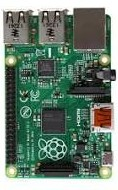
\includegraphics[width=0.7\linewidth]{ImagenesMatriz/SBC.jpg} & 
		Computadora Industrial \par\smallskip 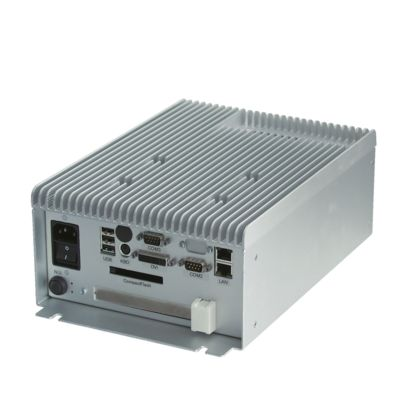
\includegraphics[width=0.9\linewidth]{ImagenesMatriz/IPC.jpg} \\ \hline
		\textbf{15. Registrar datos meteorológicos} & 
		Memoria Flash \par\smallskip 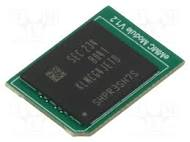
\includegraphics[width=0.7\linewidth]{ImagenesMatriz/MemoriaFLASH.jpg} & 
		MicroSD SPI \par\smallskip 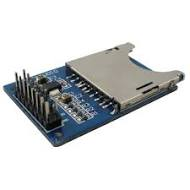
\includegraphics[width=0.7\linewidth]{ImagenesMatriz/ModuloMicroSDSPI.jpg} & 
		EEPROM I2C \par\smallskip 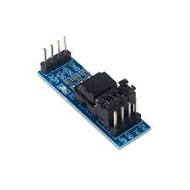
\includegraphics[width=0.7\linewidth]{ImagenesMatriz/MemoriaEEPROMI2C.jpg} \\ \hline
		\textbf{16. Procesar rutas de inspección} & 
		Microcontrolador \par\smallskip 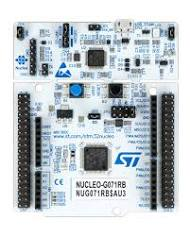
\includegraphics[width=0.7\linewidth]{ImagenesMatriz/Microcontrolador.jpg} & 
		Placa SBC \par\smallskip 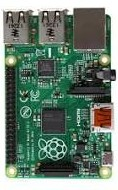
\includegraphics[width=0.7\linewidth]{ImagenesMatriz/SBC.jpg} & 
		Coprocesador GPS \par\smallskip 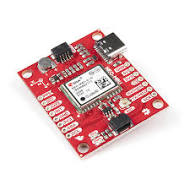
\includegraphics[width=0.9\linewidth]{ImagenesMatriz/ModuloGPSDeadReckoning.jpg} \\ \hline
		\textbf{17. Procesar posición del sistema} & 
		Microcontrolador \par\smallskip 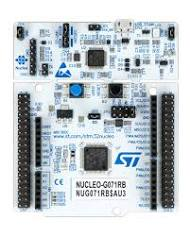
\includegraphics[width=0.7\linewidth]{ImagenesMatriz/Microcontrolador.jpg} & 
		Placa SBC \par\smallskip 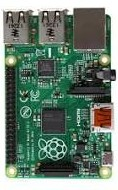
\includegraphics[width=0.7\linewidth]{ImagenesMatriz/SBC.jpg} & 
		Coprocesador GPS\par\smallskip 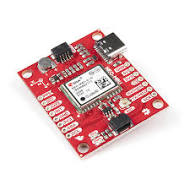
\includegraphics[width=0.9\linewidth]{ImagenesMatriz/ModuloGPSDeadReckoning.jpg} \\ \hline
	\end{xltabular}
\end{center}

\begin{itemize}
	\item \textbf{Funciones de procesamiento lógico y control de variables del sistema:} para el núcleo de estas funciones lógicas y de control, se evaluó la placa SBC, ideal para el procesamiento de datos pesados, cálculos espaciales y operaciones multitarea; el microcontrolador, que ofrece una excelente gestión de lazos cerrados en tiempo real y rutinas secuenciales con bajo consumo energético; y el PLC, que brinda máxima robustez en entornos industriales, pero cuyo tamaño y alta demanda eléctrica limitan su uso en plataformas robóticas móviles.
	
	\item \textbf{Procesar señal de obstáculo:} para la evasión de colisiones se consideró la placa SBC, que posee la capacidad de procesar nubes de puntos o mapas espaciales de forma local; el microcontrolador, útil únicamente si se emplean sensores de umbral simple con baja carga computacional; y una computadora industrial, una solución robusta con la capacidad de procesar algoritmos complejos en tiempo real y comunicarse con protocolos industriales con el PLC.
	
	\item \textbf{Registrar datos meteorológicos:} las opciones de almacenamiento contemplan el módulo MicroSD SPI, una alternativa accesible y de alta capacidad de memoria; la memoria Flash, que es muy rápida y va soldada al circuito impreso, impidiendo su extracción física manual; y la EEPROM I2C, una memoria no volátil de capacidad muy reducida, útil para guardar parámetros de configuración pero puede resultar ineficiente para el registro continuo de bases de datos climáticas.
	
	\item \textbf{Procesar rutas de inspección y Procesar posición del sistema:} para gestionar la ubicación y navegación se analizó la placa SBC, capaz de interpretar mapas complejos y algoritmos avanzados de localización simultánea; el microcontrolador, adecuado para un seguimiento de rutas simples mediante el paso de coordenadas punto a punto; y el coprocesador GPS, un circuito dedicado que se encarga exclusivamente de interpretar las tramas satelitales, liberando a la unidad central de la carga matemática de dichos cálculos espaciales.
\end{itemize}
% --- Tabla de Control (Software) ---
\begin{center}
	\footnotesize
	\begin{xltabular}{\textwidth}{|p{3.5cm}|>{\centering\arraybackslash}X|>{\centering\arraybackslash}X|>{\centering\arraybackslash}X|}
		\caption{Matriz Morfológica del Dominio de Control (Software).}
		\label{tab:matriz_control_sw} \\
		\hline
		\rowcolor[HTML]{D9E1F2} 
		\textbf{Función Parcial} & \textbf{Solución 1} & \textbf{Solución 2} & \textbf{Solución 3} \\ \hline
		\endfirsthead
		\multicolumn{4}{c}%
		{{\bfseries \tablename\ \thetable{} -- Continuación de la página anterior}} \\
		\hline
		\rowcolor[HTML]{D9E1F2} 
		\textbf{Función Parcial} & \textbf{Solución 1} & \textbf{Solución 2} & \textbf{Solución 3} \\ \hline
		\endhead
		\hline
		\endfoot
		\hline
		\endlastfoot
		% --- INICIO BLOQUE DE 8 FILAS ---
		\textbf{1. Procesar datos meteorológicos} & 
		\multirow{8}{=}{\centering Look-up table \par\vspace{0.2cm} 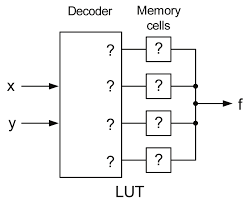
\includegraphics[width=\linewidth]{ImagenesMatriz/LookUpTables.png}} & 
		\multirow{8}{=}{\centering Algoritmo por ecuación \par\vspace{0.2cm} 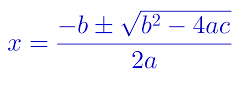
\includegraphics[width=0.8\linewidth]{ImagenesMatriz/AlgoritmoEcuacion.png}} & 
		\multirow{8}{=}{\centering Algoritmo de promedio \par\vspace{0.2cm} 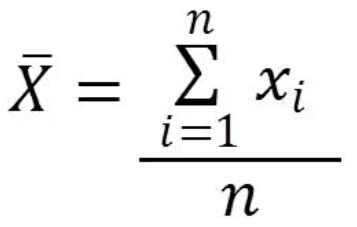
\includegraphics[width=\linewidth]{ImagenesMatriz/AlgoritmoPromedio.png}} \\ \cline{1-1}
		\textbf{2. Procesar temperatura del gestionador} & & & \\ \cline{1-1}
		\textbf{3. Procesar nivel energía del gestionador} & & & \\ \cline{1-1}
		\textbf{4. Procesar estado energía del gestionador} & & & \\ \cline{1-1}
		\textbf{5. Procesar velocidad de traslación} & & & \\ \cline{1-1}
		\textbf{6. Procesar orientación de plataforma} & & & \\ \cline{1-1}
		\textbf{7. Procesar posición de plataforma} & & & \\ \cline{1-1}
		\textbf{8. Controlar estado energía del gestionador} & & & \\ \hline
		\textbf{9. Controlar movimiento de traslación} \vspace{1cm}& 
		\multirow{3}{=}{\centering Control SMC \par\vspace{0.2cm} 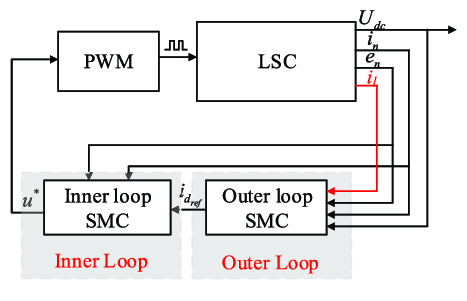
\includegraphics[width=\linewidth]{ImagenesMatriz/ControlSMC.png}} & 
		\multirow{3}{=}{\centering Control PID \par\vspace{0.2cm} 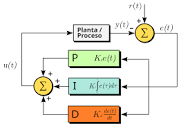
\includegraphics[width=\linewidth]{ImagenesMatriz/ControlPID.png}} & 
		\multirow{3}{=}{\centering Lógica Difusa \par\vspace{0.2cm} 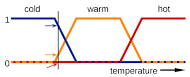
\includegraphics[width=\linewidth]{ImagenesMatriz/LogicaDifusa.png}} \\ \cline{1-1}
		\textbf{10. Controlar movimiento de orientación de plataforma} & & & \\ \cline{1-1}
		\textbf{11. Controlar posicionamiento de plataforma} & & & \\ \hline
		% --- FILAS INDIVIDUALES ---
		\textbf{12. Procesar dirección de traslación} & 
		Controlador Stanley paralelo \par\smallskip 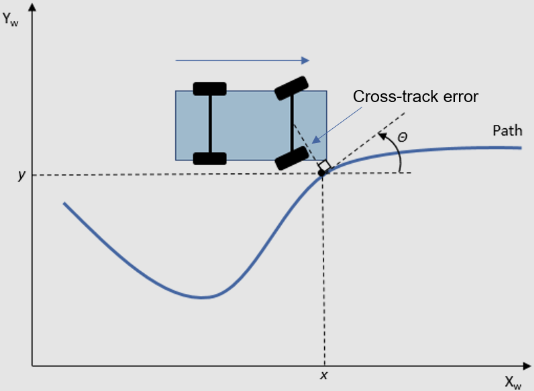
\includegraphics[width=\linewidth]{ImagenesMatriz/StanleyParalelo.png} & 
		Algoritmo Pure Pursuit \par\smallskip 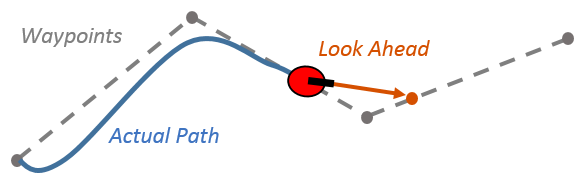
\includegraphics[width=\linewidth]{ImagenesMatriz/PurePursuit.png} & 
		Algoritmo Vector Pursuit\par\smallskip 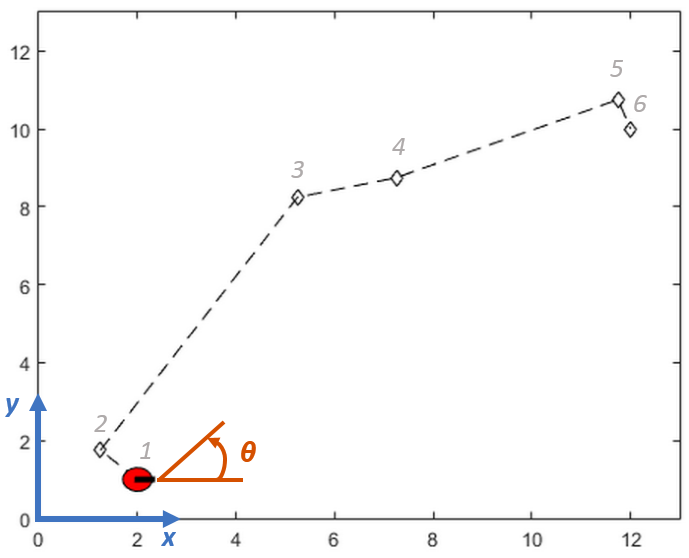
\includegraphics[width=\linewidth]{ImagenesMatriz/VectorPursuit.png} \\ \hline
		\textbf{13. Procesar señal de obstáculo} & 
		Comparación por umbrales y ventanas de tiempo \par\smallskip 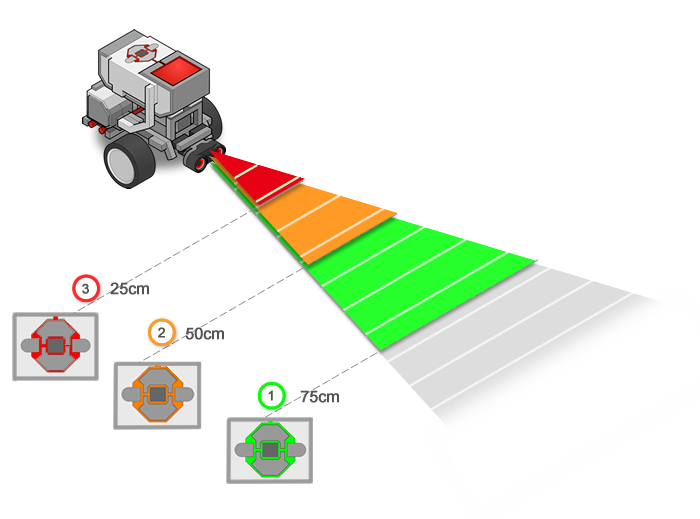
\includegraphics[width=\linewidth]{ImagenesMatriz/Thresholding.png} & 
		Flujo óptico \par\smallskip 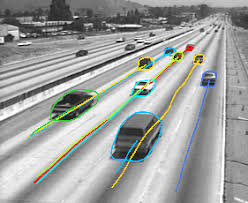
\includegraphics[width=\linewidth]{ImagenesMatriz/OpticalFlow.jpg} & 
		Agrupamiento y segmentación \par\smallskip 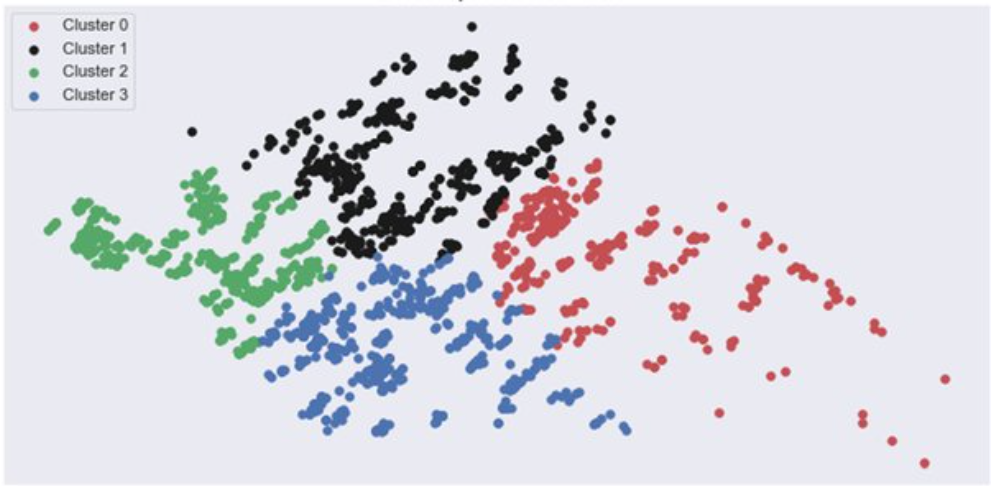
\includegraphics[width=\linewidth]{ImagenesMatriz/AgrupamientoSegmentacion.png} \\ \hline
		\textbf{14. Registrar datos meteorológicos} & 
		Buffer de almacenamiento asíncrono \par\smallskip 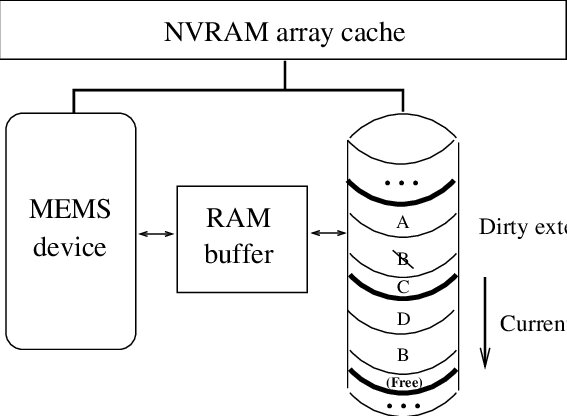
\includegraphics[width=\linewidth]{ImagenesMatriz/AsyncMemoria.jpg} & 
		Acceso directo a sistemas de archivos embebidos \par\smallskip 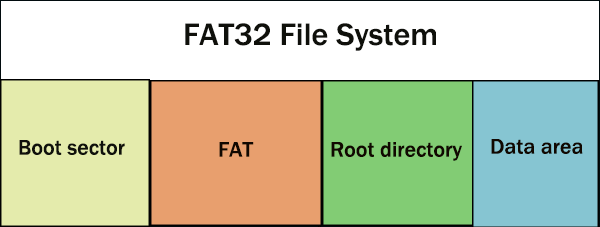
\includegraphics[width=\linewidth]{ImagenesMatriz/FAT32.png} & 
		Motores de data bases \par\smallskip 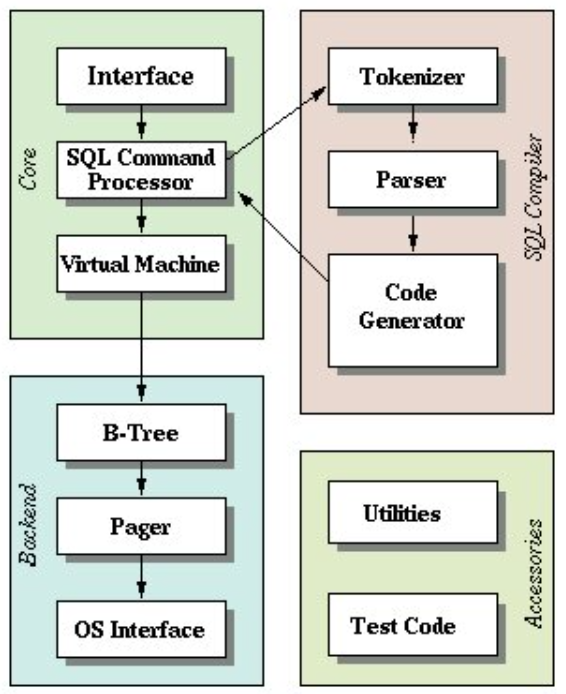
\includegraphics[width=\linewidth]{ImagenesMatriz/SQLite.png} \\ \hline
		\textbf{15. Procesar rutas de inspección} \vspace{1.5cm} & 
		\multirow{2}{=}{\centering A - Navigation por mapas de nodos \par\smallskip 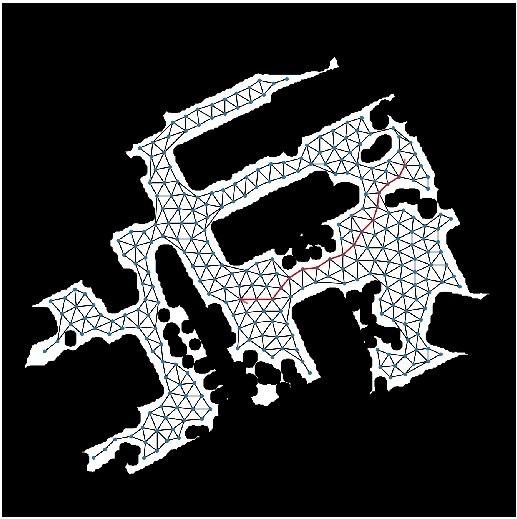
\includegraphics[width=\linewidth]{ImagenesMatriz/RoadmapNodes.jpg}} & 
		\multirow{2}{=}{\centering B - Navegación por histograma de campo vectorial\par\smallskip 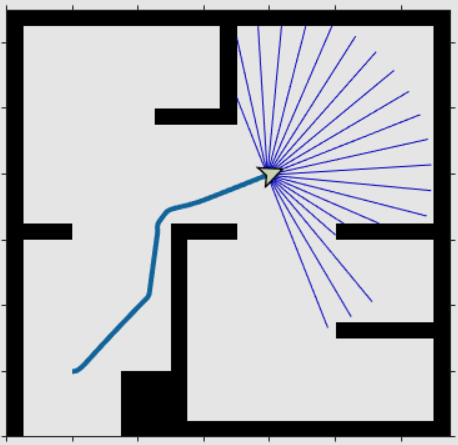
\includegraphics[width=\linewidth]{ImagenesMatriz/VectorFieldNav.png}} & 
		\multirow{2}{=}{\centering C - Navegación por mapas de costo\par\smallskip 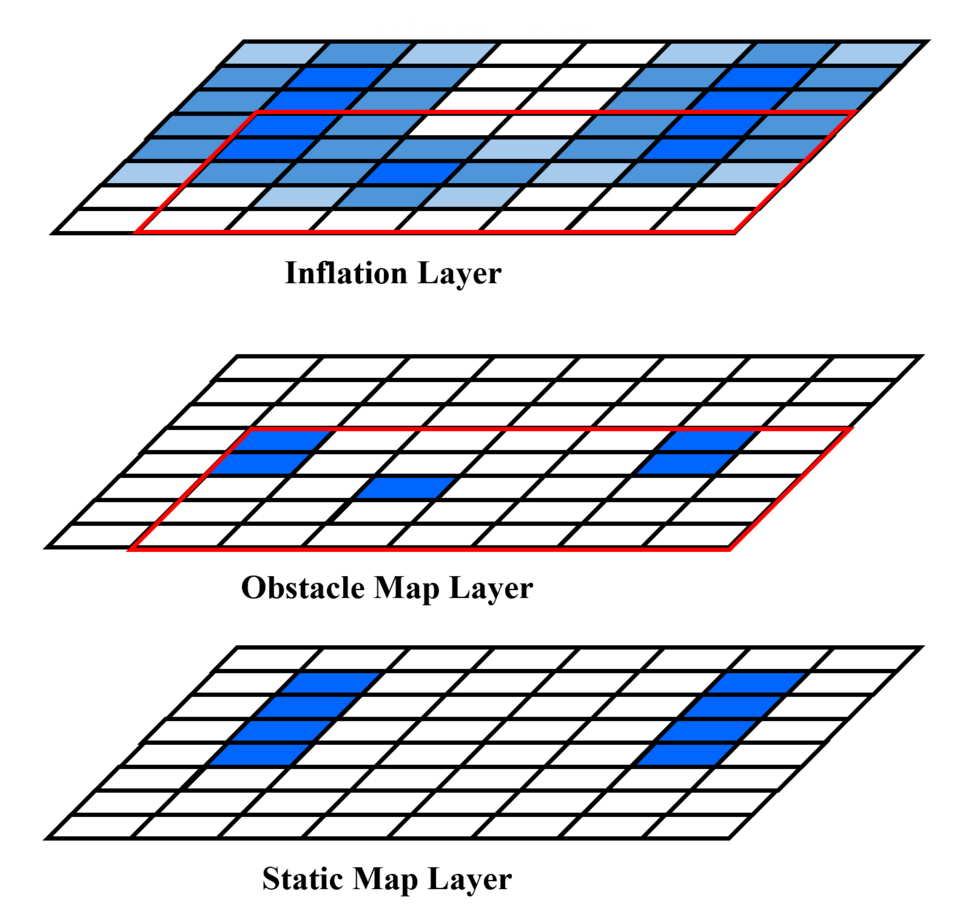
\includegraphics[width=\linewidth]{ImagenesMatriz/Costmap.png}} \\ \cline{1-1}
		\textbf{16. Procesar posición del sistema} \vspace{1.5cm} & & & \\ \hline
	\end{xltabular}
\end{center}

\begin{itemize}
	\item \textbf{Funciones de procesamiento lógico de señales y evaluación del estado general:} para el procesamiento lógico de las señales y la evaluación del estado general, se evaluó el algoritmo por ecuación, que ofrece una conversión matemática exacta pero puede demandar mayor tiempo de procesamiento en el microcontrolador; la look-up table (tabla de búsqueda), que garantiza una ejecución muy rápida al precalcular los valores a costa de ocupar mayor espacio en la memoria; y el algoritmo de promedio, una opción simple que ayuda a filtrar el ruido eléctrico de las lecturas continuas, aunque puede presentar cierto retraso temporal frente a cambios dinámicos rápidos.
	
	\item \textbf{Controlar movimiento de traslación, Controlar movimiento de orientación de plataforma y Controlar posicionamiento de plataforma :} para los lazos de control de los actuadores físicos, se consideró el control PID, que representa el estándar de la industria por su simplicidad y fiabilidad para mantener posiciones o velocidades estables; la lógica difusa, útil para manejar las no linealidades mecánicas mediante reglas lógicas sin requerir un modelo matemático exacto, pero cuya sintonización es compleja; y el control SMC, que destaca por su altísima robustez frente a perturbaciones externas o irregularidades del terreno, aunque puede generar un esfuerzo de control discontinuo y desgaste mecánico prematuro.
	
	\item \textbf{Procesar dirección de traslación:} para guiar el desplazamiento del vehículo, se analizó el algoritmo Pure Pursuit, un método geométrico de seguimiento de ruta sencillo y confiable, pero que tiende a recortar las curvas si la distancia de visión no se ajusta correctamente; el algoritmo Vector Pursuit, que mejora la precisión geométrica al considerar tanto la posición como la orientación del objetivo a alcanzar; y el controlador Stanley paralelo, el cual minimiza eficazmente el error lateral respecto a la trayectoria deseada y se adapta de forma óptima a las variaciones de velocidad del vehículo sobre el terreno.
	
	\item \textbf{Procesar señal de obstáculo:} para la detección y evasión de elementos en la vía, se evaluó la comparación por umbrales y ventanas de tiempo, que exige una carga computacional mínima pero es susceptible a generar falsos positivos por ruido; el agrupamiento y segmentación, ideal para procesar nubes de puntos espaciales separando eficazmente el suelo llano de los obstáculos reales con alta fiabilidad; y el flujo óptico, que detecta el movimiento relativo mediante secuencias de imágenes de cámara, aunque su eficacia disminuye drásticamente en entornos con iluminación variable o alto nivel de polvo.
	
	\item \textbf{Registrar datos meteorológicos:} para el resguardo de la información climática, se propuso el acceso directo a sistemas de archivos embebidos, que permite una escritura secuencial simple pero puede bloquear temporalmente el procesador principal; los motores de bases de datos, que estructuran la información para facilitar consultas complejas y búsquedas a cambio de una alta exigencia de memoria RAM; y el buffer de almacenamiento asíncrono, que garantiza que los datos se recopilen y guarden en segundo plano sin interrumpir los tiempos de ejecución de los ciclos críticos de control del robot.
	
	\item \textbf{Procesar rutas de inspección y Procesar posición del sistema:} para planificar y seguir el recorrido dentro del parque fotovoltaico, se consideró la navegación por mapas de nodos, que requiere escasa memoria al estructurar la planta solar simplemente como un grafo de puntos secuenciales a visitar; la navegación por mapas de costo, que permite representar áreas seguras, zonas de riesgo y obstáculos como gradientes para un desplazamiento mucho más seguro; y la navegación por histograma de campo vectorial, excelente para calcular trayectorias y evadir obstáculos locales de forma fluida y en tiempo real.
\end{itemize}

\subsection{Dominio de Comunicación}
% Espacio para tabla de Comunicación
\begin{center}
	\footnotesize
	\begin{xltabular}{\textwidth}{|p{3.5cm}|>{\raggedright\arraybackslash}X|>{\raggedright\arraybackslash}X|>{\raggedright\arraybackslash}X|}
		\caption{Matriz Morfológica del Dominio de Comunicación.}
		\label{tab:matriz_comunicacion} \\
		\hline
		\rowcolor[HTML]{D9E1F2} 
		\textbf{Función Parcial} & \textbf{Solución 1} & \textbf{Solución 2} & \textbf{Solución 3} \\ \hline
		\endfirsthead
		\multicolumn{4}{c}%
		{{\bfseries \tablename\ \thetable{} -- Continuación de la página anterior}} \\
		\hline
		\rowcolor[HTML]{D9E1F2} 
		\textbf{Función Parcial} & \textbf{Solución 1} & \textbf{Solución 2} & \textbf{Solución 3} \\ \hline
		\endhead
		\hline
		\endfoot
		\hline
		\endlastfoot
		% --- INICIO BLOQUE 1-2 ---
		\textbf{1. Procesar señal GPS} \vspace{0.8cm} & 
		\multirow{2}{=}{ Trilaterización \par\smallskip 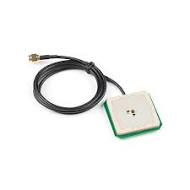
\includegraphics[width=0.7\linewidth]{ImagenesMatriz/AntenaGNSS.jpg}} & 
		\multirow{2}{=}{ Trilaterización con Dead Reckoning \par\smallskip 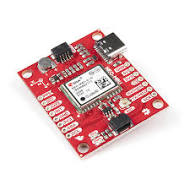
\includegraphics[width=0.7\linewidth]{ImagenesMatriz/ModuloGPSDeadReckoning.jpg}} & 
		\multirow{2}{=}{ Medición de fase de onda \par\smallskip 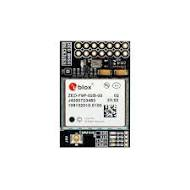
\includegraphics[width=0.7\linewidth]{ImagenesMatriz/ModuloFasePortadora.jpg}} \\ \cline{1-1}
		\textbf{2. Procesar señal de mando} \vspace{0.8cm} & & & \\ \hline
		% --- FIN BLOQUE 1-2 ---
		% --- INICIO BLOQUE 3-4 ---
		\textbf{3. Transmitir estado de telemetría} \vspace{0.8cm} & 
		\multirow{2}{=}{Protocolo MQTT +Wi-Fi\par\smallskip 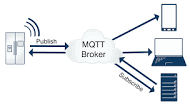
\includegraphics[width=\linewidth]{ImagenesMatriz/ProtocoloMQTT.png}} & 
		\multirow{2}{=}{Módulo LoRa \par\smallskip 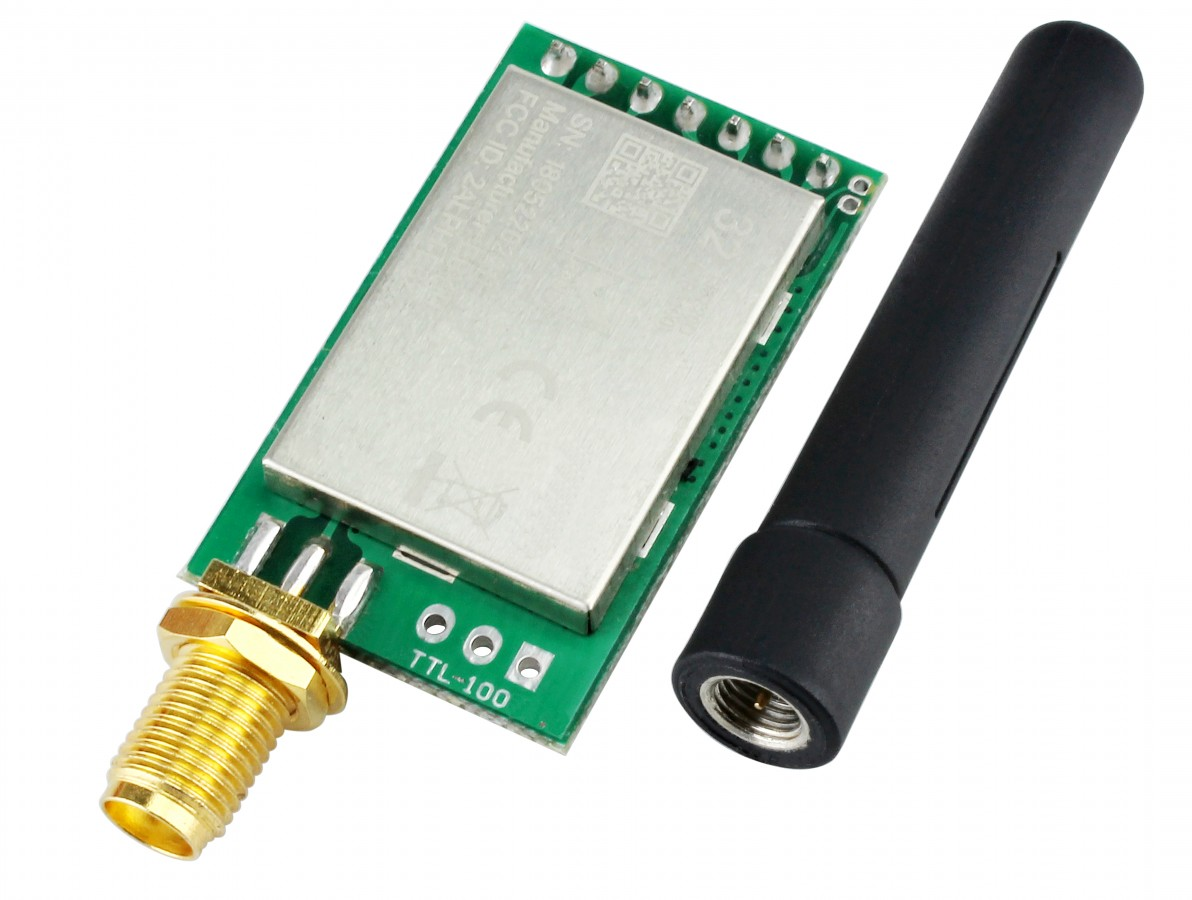
\includegraphics[width=0.7\linewidth]{ImagenesMatriz/ModuloLoRa.jpg}} & 
		\multirow{2}{=}{Celular LTE-M \par\smallskip 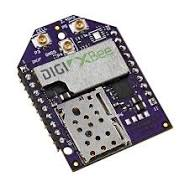
\includegraphics[width=0.7\linewidth]{ImagenesMatriz/CelularLTEM.jpg}} \\ \cline{1-1}
		\textbf{4. Transmitir datos meteorológicos} \vspace{0.2cm}& & & \\ \hline
		% --- FIN BLOQUE 3-4 ---
	\end{xltabular}
\end{center}

\begin{itemize}
	\item \textbf{Procesar señal GPS y Procesar señal de mando:} para el cálculo de la ubicación y el procesamiento de instrucciones se evaluó la trilateración, un método de posicionamiento estándar y económico basado en la distancia a los satélites, aunque vulnerable a la pérdida de conexión; la medición de fase de onda (tipo RTK), que otorga una alta precisión centimétrica pero requiere el uso de una estación base y mayor capacidad de procesamiento; y la trilateración con Dead Reckoning, que combina los datos satelitales con la odometría interna del vehículo para mantener la estimación exacta de la posición incluso cuando la señal satelital se bloquea al transitar bajo los paneles solares.
	
	\item \textbf{Transmitir estado de telemetría y Transmitir datos meteorológicos:} para la emisión de la información y alertas hacia el exterior se analizó el módulo LoRa, que permite la transmisión de datos a largas distancias con un consumo energético mínimo, siendo ideal para las grandes extensiones de terreno de las plantas solares; el celular LTE-M, que ofrece una conexión directa a la nube con un mayor ancho de banda, pero depende de la disponibilidad y estabilidad de la cobertura de la red operadora local; y la combinación del protocolo MQTT + Wi-Fi, que garantiza una alta velocidad para la transferencia de paquetes, pero cuyo alcance limitado exigiría instalar una costosa red de múltiples puntos de acceso a lo largo de todo el terreno.
\end{itemize}

\subsection{Dominio de Interfaz}
% Espacio para tabla de Interfaz

\begin{center}
	\footnotesize
	\begin{xltabular}{\textwidth}{|p{3.5cm}|>{\raggedright\arraybackslash}X|>{\raggedright\arraybackslash}X|>{\raggedright\arraybackslash}X|}
		\caption{Matriz Morfológica del Dominio de Interfaz.}
		\label{tab:matriz_interfaz} \\
		\hline
		\rowcolor[HTML]{D9E1F2} 
		\textbf{Función Parcial} & \textbf{Solución 1} & \textbf{Solución 2} & \textbf{Solución 3} \\ \hline
		\endfirsthead
		\multicolumn{4}{c}%
		{{\bfseries \tablename\ \thetable{} -- Continuación de la página anterior}} \\
		\hline
		\rowcolor[HTML]{D9E1F2} 
		\textbf{Función Parcial} & \textbf{Solución 1} & \textbf{Solución 2} & \textbf{Solución 3} \\ \hline
		\endhead
		\hline
		\endfoot
		\hline
		\endlastfoot
		% --- INICIO BLOQUE 1-4 ---
		\textbf{1. Recibir señal de radiación} & 
		\multirow{4}{=}{Conector circular roscado \par\smallskip 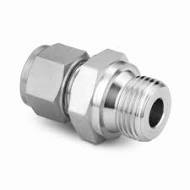
\includegraphics[width=0.8\linewidth]{ImagenesMatriz/ConectorRoscado.jpg}} & 
		\multirow{4}{=}{Borna con resorte interno \par\smallskip 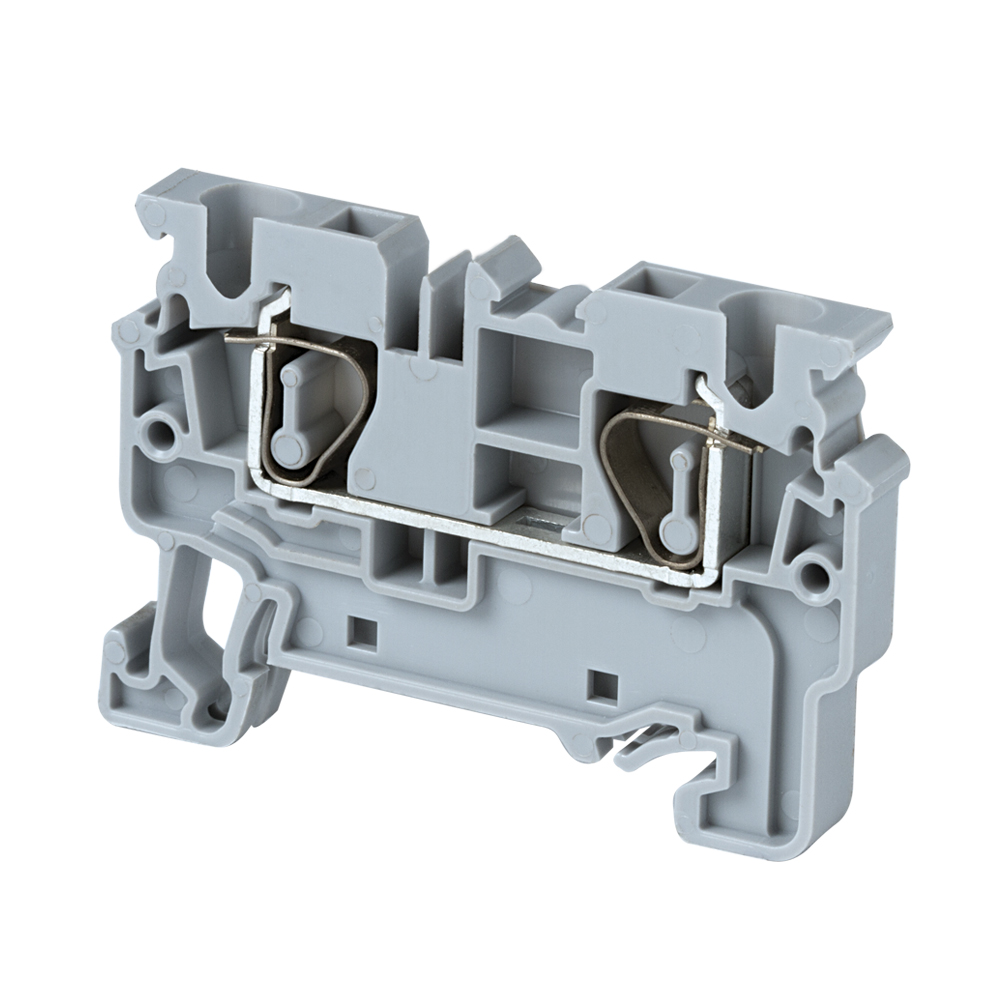
\includegraphics[width=0.8\linewidth]{ImagenesMatriz/BornaResorte.jpg}} & 
		\multirow{4}{=}{Conector Deutsch \par\smallskip 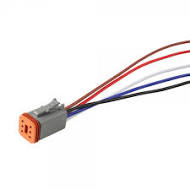
\includegraphics[width=\linewidth]{ImagenesMatriz/ConectorDeutsch.jpg}} \\ \cline{1-1}
		\textbf{2. Recibir señal de temperatura} & & & \\ \cline{1-1}
		\textbf{3. Recibir señal de velocidad viento} & & & \\ \cline{1-1}
		\textbf{4. Recibir señal de humedad} & & & \\ \hline
		% --- FIN BLOQUE 1-4 ---
		% --- INICIO BLOQUE 5-6 ---
		\textbf{5. Mostrar alerta obstáculo} \vspace{1cm}& 
		\multirow{2}{=}{Buzzer \par\smallskip 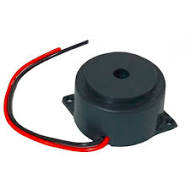
\includegraphics[width=0.8\linewidth]{ImagenesMatriz/Buzzer.jpg}} & 
		\multirow{2}{=}{Pantalla LCD \par\smallskip 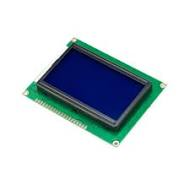
\includegraphics[width=0.8\linewidth]{ImagenesMatriz/PantallaLCD.jpg}} & 
		\multirow{2}{=}{Sirena LED \par\smallskip 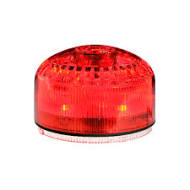
\includegraphics[width=0.8\linewidth]{ImagenesMatriz/SirenaLED.jpg}} \\ \cline{1-1}
		\textbf{6. Mostrar alerta energía} & & & \\ \hline
		% --- FIN BLOQUE 5-6 ---
		
		
		% --- INICIO BLOQUE 7-8 ---
		\textbf{7. Mostrar estado energía} \vspace{1cm}& 
		\multirow{2}{=}{LEDs indicadores \par\smallskip 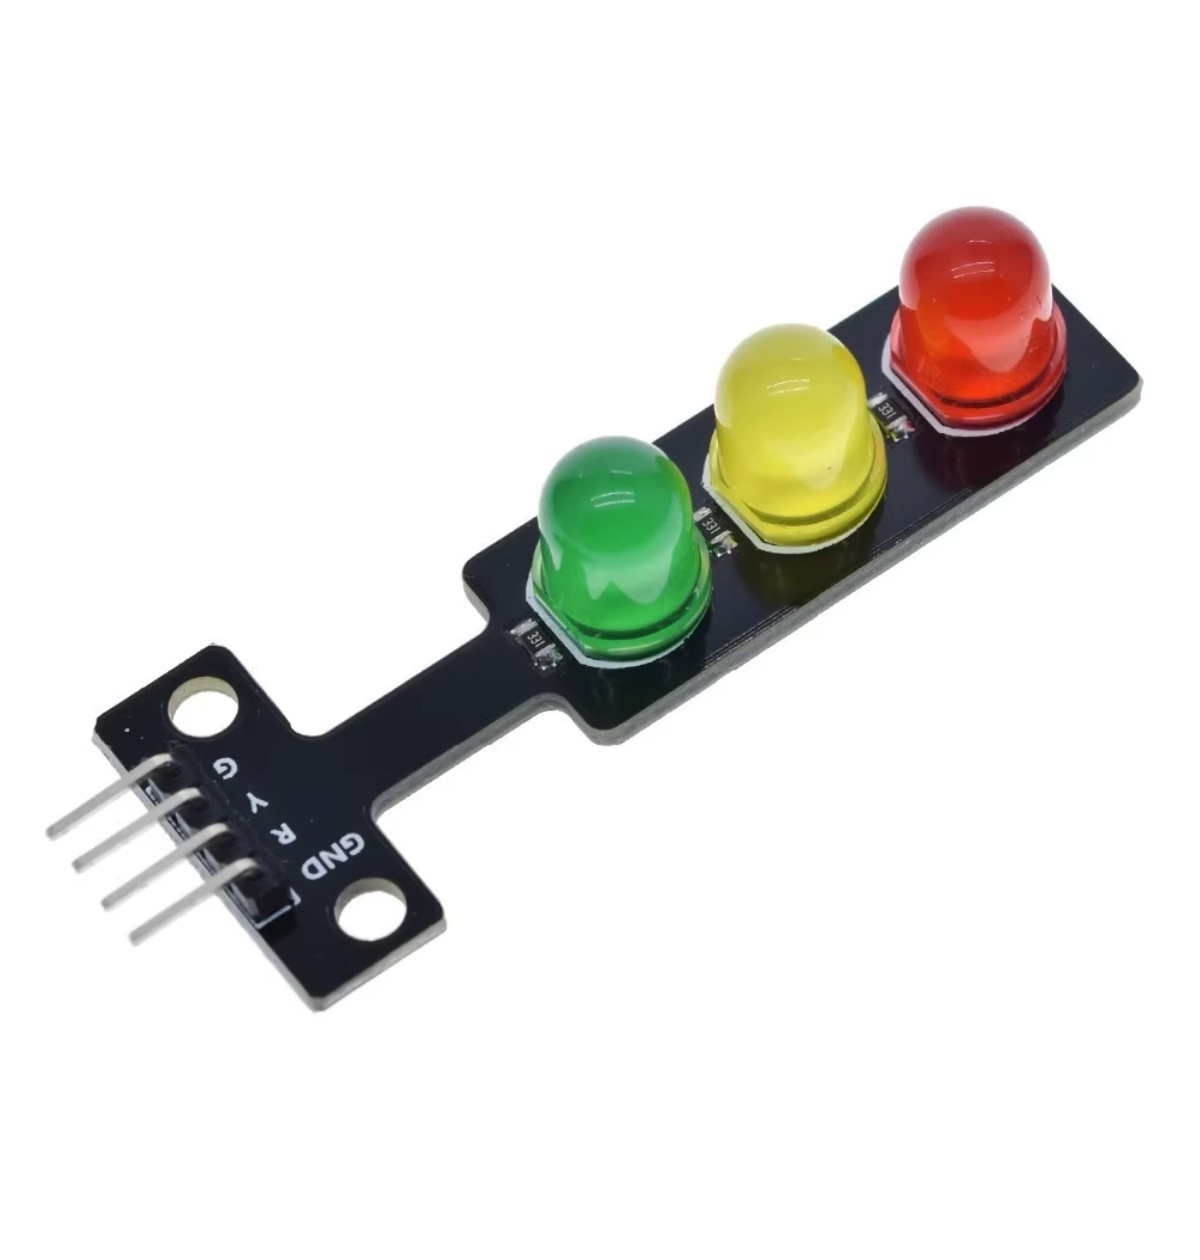
\includegraphics[width=0.8\linewidth]{ImagenesMatriz/LEDIndicador.jpeg}} & 
		\multirow{2}{=}{Pantalla LCD \par\smallskip 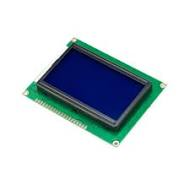
\includegraphics[width=0.8\linewidth]{ImagenesMatriz/PantallaLCD.jpg}} & 
		\multirow{2}{=}{Pantalla HMI \par\smallskip 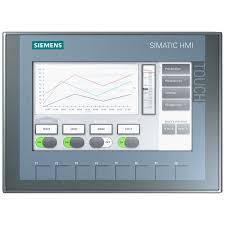
\includegraphics[width=0.8\linewidth]{ImagenesMatriz/PantallaHMI.jpg}} \\ \cline{1-1}
		\textbf{8. Mostrar estado operativo} & & & \\ \hline
		% --- FIN BLOQUE 7-8 ---
	\end{xltabular}
\end{center}

\begin{itemize}
	\item \textbf{Funciones de recepción de señales de instrumentación meteorológica:} para la conexión de los sensores externos se evaluó la borna con resorte interno, que permite un ensamblaje rápido del cableado pero es vulnerable a desconexiones por las continuas vibraciones del robot sobre el terreno; el conector circular roscado, que garantiza un acople industrial firme y con alta protección contra el polvo y la humedad propia del entorno de la planta; y el conector Deutsch, reconocido por su excelente sello hermético en vehículos, pero que exige herramientas especiales de crimpado que dificultan su mantenimiento en campo.
	
	\item \textbf{Mostrar alerta obstáculo y Mostrar alerta energía:} para la emisión de advertencias críticas se consideró el buzzer, que proporciona una alarma sonora inmediata y efectiva con un consumo de energía mínimo para prevenir colisiones; la sirena LED, que entrega un aviso combinado de alta potencia pero resulta sobredimensionada y representa un gasto energético excesivo para el tamaño del vehículo; y la pantalla LCD, que si bien detalla el tipo de error, es ineficiente como mecanismo de alerta rápida ya que requiere que el personal se acerque al equipo para poder leerla.
	
	\item \textbf{Mostrar estado energía y Mostrar estado operativo:} para la supervisión local y directa del sistema se analizó la pantalla LCD, útil para mostrar valores exactos pero propensa a reflejos bajo la luz directa del sol; la pantalla HMI, que ofrece una interacción táctil avanzada a cambio de una mayor fragilidad ante impactos and un alto consumo de las baterías; y los LEDs indicadores, que representan la opción más robusta y eficiente al codificar los estados operativos mediante colores simples, lo que permite una lectura rápida a la distancia prescindiendo de pantallas de alto consumo.
\end{itemize}

\subsection{Dominio de Actuadores}
% Espacio para tabla de Actuadores

\begin{center}
	\footnotesize
	\begin{xltabular}{\textwidth}{|p{3.5cm}|>{\raggedright\arraybackslash}X|>{\raggedright\arraybackslash}X|>{\raggedright\arraybackslash}X|}
		\caption{Matriz Morfológica del Dominio de Actuadores.}
		\label{tab:matriz_actuadores} \\
		\hline
		\rowcolor[HTML]{D9E1F2} 
		\textbf{Función Parcial} & \textbf{Solución 1} & \textbf{Solución 2} & \textbf{Solución 3} \\ \hline
		\endfirsthead
		
		\multicolumn{4}{c}%
		{{\bfseries \tablename\ \thetable{} -- Continuación de la página anterior}} \\
		\hline
		\rowcolor[HTML]{D9E1F2} 
		\textbf{Función Parcial} & \textbf{Solución 1} & \textbf{Solución 2} & \textbf{Solución 3} \\ \hline
		\endhead
		
		\hline
		\endfoot
		
		\hline
		\endlastfoot
		
		\textbf{1. Accionar movimiento de traslación} 
		& Motor de Cubo de Rueda \par\smallskip 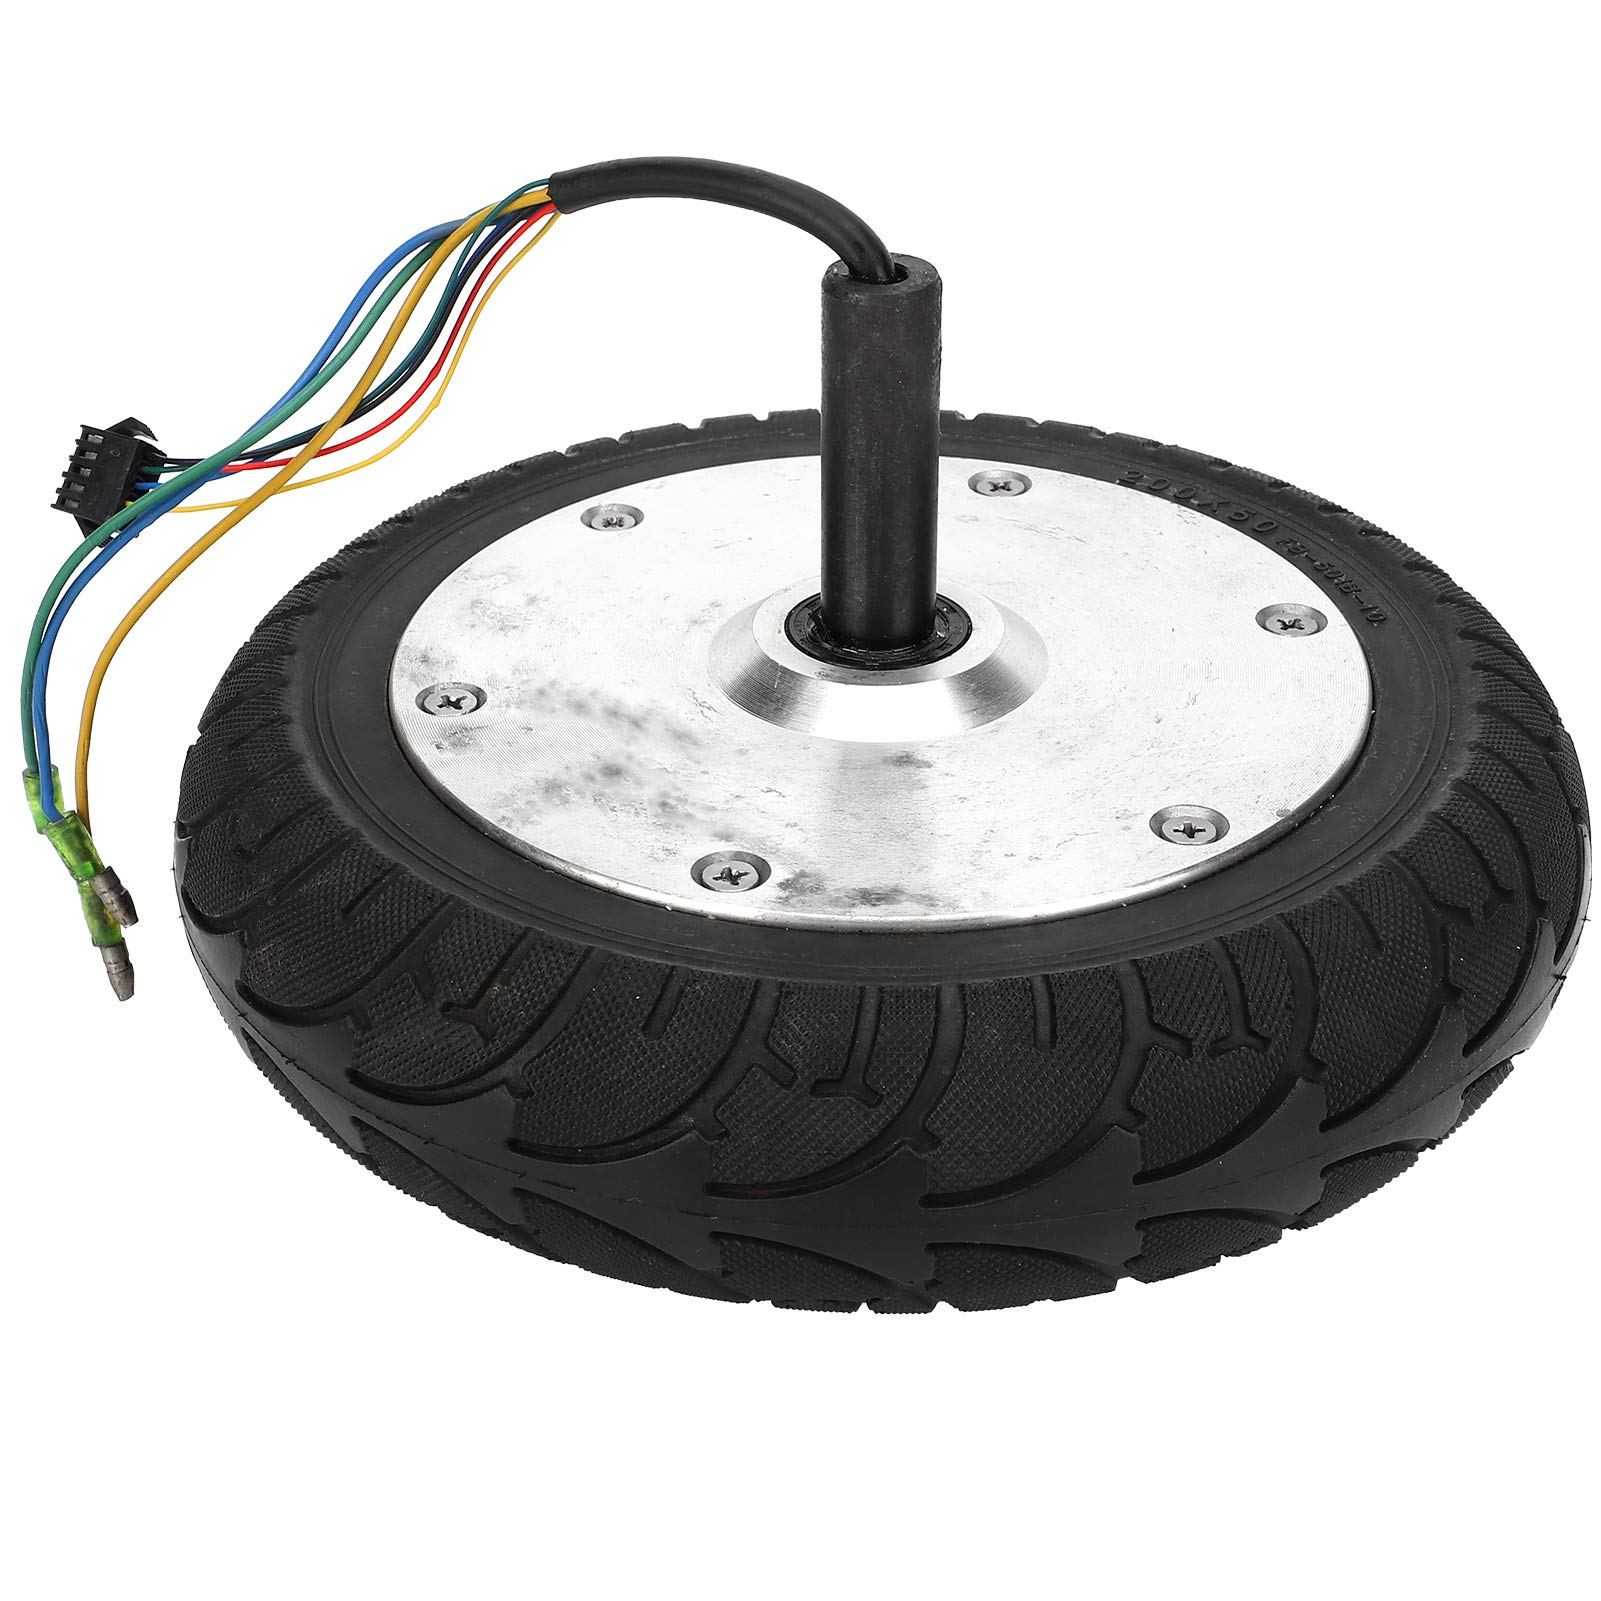
\includegraphics[width=\linewidth]{ImagenesMatriz/MotorCuboDeRueda.jpg} & Servomotor Brushless DC \par\smallskip 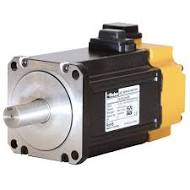
\includegraphics[width=\linewidth]{ImagenesMatriz/ServomotorBrushless.jpg} &  Motorreductor DC  \par\smallskip 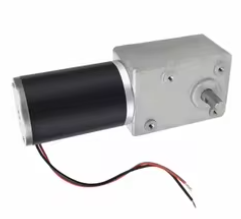
\includegraphics[width=\linewidth]{ImagenesMatriz/MotorreductorDC.png} \\ \hline
		\textbf{2. Accionar orientación de la plataforma} & 
		Microservo digital \par\smallskip 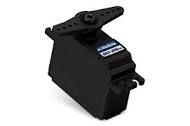
\includegraphics[width=\linewidth]{ImagenesMatriz/Miniservo.jpg}& Servomotor Brushless DC \par\smallskip 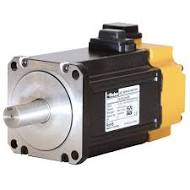
\includegraphics[width=\linewidth]{ImagenesMatriz/ServomotorBrushless.jpg}& 	Motor paso a paso NEMA \par\smallskip 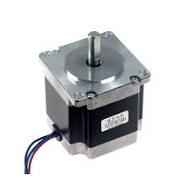
\includegraphics[width=\linewidth]{ImagenesMatriz/MotorNEMA.jpg}\\ \hline
		\textbf{3. Accionar posición de la plataforma} &
		Actuador lineal \par\smallskip 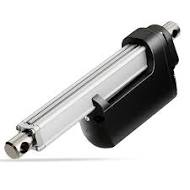
\includegraphics[width=\linewidth]{ImagenesMatriz/ActuadorLineal.jpg} & Servomotor Brushless DC \par\smallskip 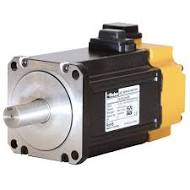
\includegraphics[width=\linewidth]{ImagenesMatriz/ServomotorBrushless.jpg}& Actuador lineal \par\smallskip 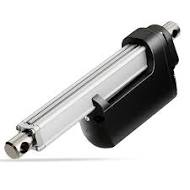
\includegraphics[width=\linewidth]{ImagenesMatriz/ActuadorLineal.jpg}\\ \hline
		
	\end{xltabular}
\end{center}


\begin{itemize}
	\item \textbf{Accionar movimiento de traslación:} para la tracción principal del vehículo sobre el terreno, se evaluó el motor paso a paso NEMA, que ofrece un alto torque a bajas velocidades y un avance preciso, aunque con un consumo energético constante y elevado; el servomotor Brushless DC, que brinda una alta eficiencia, vida útil prolongada y control exacto en lazo cerrado para la navegación, pero con mayor costo y complejidad de implementación; y el motor DC estándar, que representa una opción económica y de control sencillo, pero es susceptible a un mayor desgaste mecánico y posee menor precisión para sortear las irregularidades del suelo.
	
	\item \textbf{Accionar orientación de la plataforma:} para el ajuste del ángulo de los instrumentos de medición climática, se consideró el motor paso a paso NEMA, que asegura una excelente retención estática y precisión para mantener la inclinación deseada frente a las vibraciones del entorno; el servomotor Brushless DC, que proporciona un control angular de gran exactitud pero resulta técnica y económicamente sobredimensionado para sostener una carga estática; y el microservo digital, una alternativa muy compacta y de control directo, pero cuya transmisión y engranajes internos pueden ser vulnerables a daños mecánicos bajo los esfuerzos continuos de la plataforma.
	
	\item \textbf{Accionar posición de la plataforma:} Se evaluó el servomotor Brushless DC, que proporciona alta precisión pero exige un consumo eléctrico continuo para mantener la carga estática y el actuador lineal, con una capacidad de ejecutar el movimiento rectilíneo directo y retener mecánicamente la elevación sin consumo de energía constante.

\end{itemize}
\subsection{Dominio Mecánico}
% Espacio para tabla de Mecánico
\begin{center}
	\footnotesize
	\begin{xltabular}{\textwidth}{|p{3.5cm}|>{\raggedright\arraybackslash}X|>{\raggedright\arraybackslash}X|>{\raggedright\arraybackslash}X|}
		\caption{Matriz Morfológica del Dominio Mecánico.}
		\label{tab:matriz_mecanico} \\
		\hline
		\rowcolor[HTML]{D9E1F2} 
		\textbf{Función Parcial} & \textbf{Solución 1} & \textbf{Solución 2} & \textbf{Solución 3} \\ \hline
		\endfirsthead
		\multicolumn{4}{c}%
		{{\bfseries \tablename\ \thetable{} -- Continuación de la página anterior}} \\
		\hline
		\rowcolor[HTML]{D9E1F2} 
		\textbf{Función Parcial} & \textbf{Solución 1} & \textbf{Solución 2} & \textbf{Solución 3} \\ \hline
		\endhead
		\hline
		\endfoot
		\hline
		\endlastfoot
		% --- INICIO BLOQUE 1-2 ---
		\textbf{1. Soportar plataforma de medición} \vspace{1cm}& 
		\multirow{2}{=}{Piezas de MDF \par\smallskip 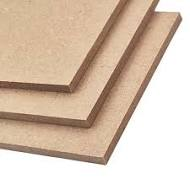
\includegraphics[width=0.8\linewidth]{ImagenesMatriz/PiezasMDF.jpg}} & 
		\multirow{2}{=}{Perfil V-Slot \par\smallskip 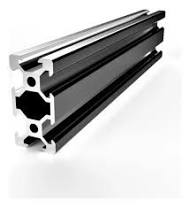
\includegraphics[width=0.8\linewidth]{ImagenesMatriz/Vslot.jpg}} & 
		\multirow{2}{=}{Chapas de Acero \par\smallskip 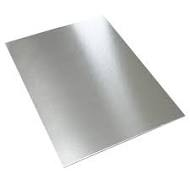
\includegraphics[width=0.8\linewidth]{ImagenesMatriz/ChapaAcero.jpg}} \\ \cline{1-1}
		\textbf{2. Soportar componentes} & & & \\ \hline
		\textbf{3. Proteger componentes} \vspace{1cm}& 
		\multirow{3}{=}{Carcasa impresa en 3D \par\smallskip 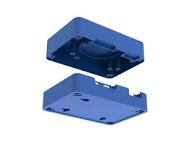
\includegraphics[width=0.8\linewidth]{ImagenesMatriz/Carcasa3D.jpg}} & 
		\multirow{3}{=}{Caja de chapa de aluminio \par\smallskip 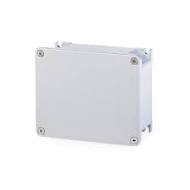
\includegraphics[width=0.8\linewidth]{ImagenesMatriz/CajaChapaAluminio.jpg}} & 
		\multirow{3}{=}{Caja de acero inoxidable \par\smallskip 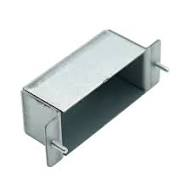
\includegraphics[width=0.8\linewidth]{ImagenesMatriz/CajaChapaAcero.jpg}} \\ \cline{1-1}
		\textbf{4. Alojar gestionador} & & & \\ \cline{1-1}
		\textbf{5. Alojar memoria externa} & & & \\ \hline
		\textbf{6. Generar movimiento de traslación} & 
		Ruedas onmidireccionales \par\smallskip 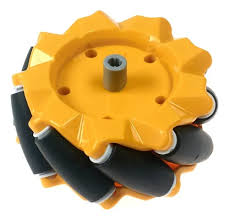
\includegraphics[width=\linewidth]{ImagenesMatriz/RuedaOnmidireccional.jpg} & 
		Tracción diferencial (4 ruedas) \par\smallskip 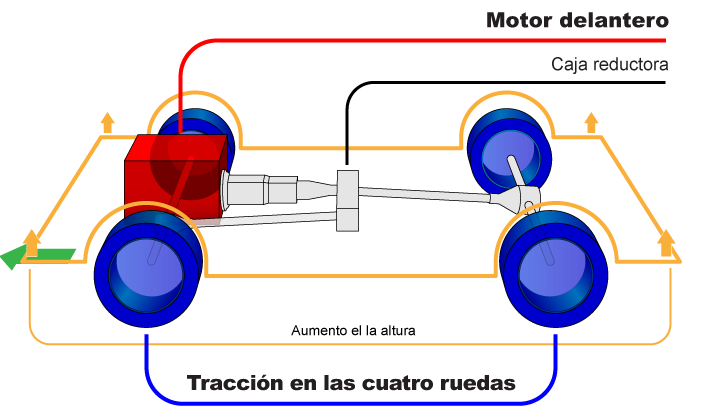
\includegraphics[width=\linewidth]{ImagenesMatriz/RuedasTraccionDiferencial.png} & 
		Ruedas con tracción de oruga \par\smallskip 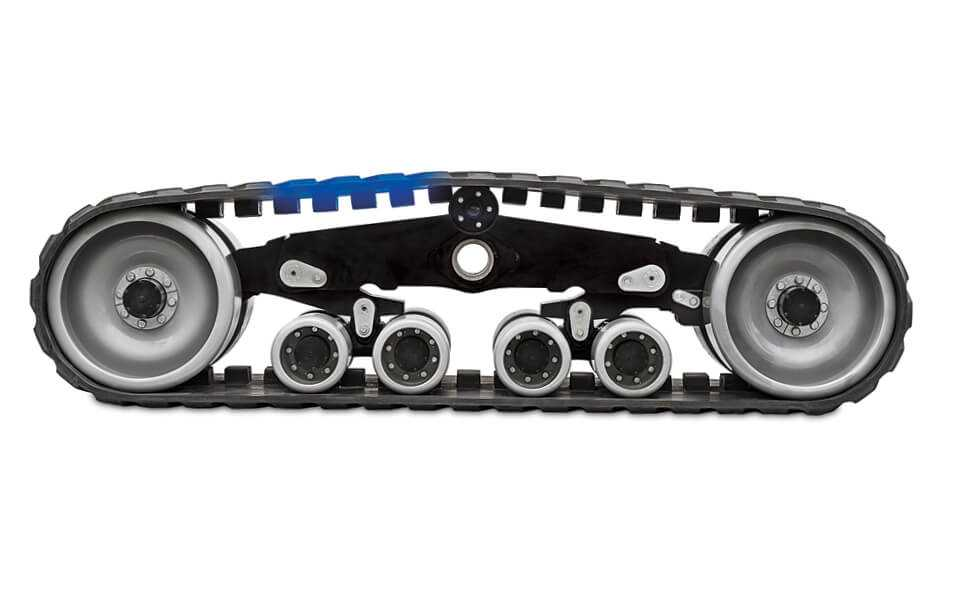
\includegraphics[width=\linewidth]{ImagenesMatriz/RuedasTraccionOruga.jpg} \\ \hline
		\textbf{7. Orientar plataforma} & 
		Eje acoplado a motor \par\smallskip 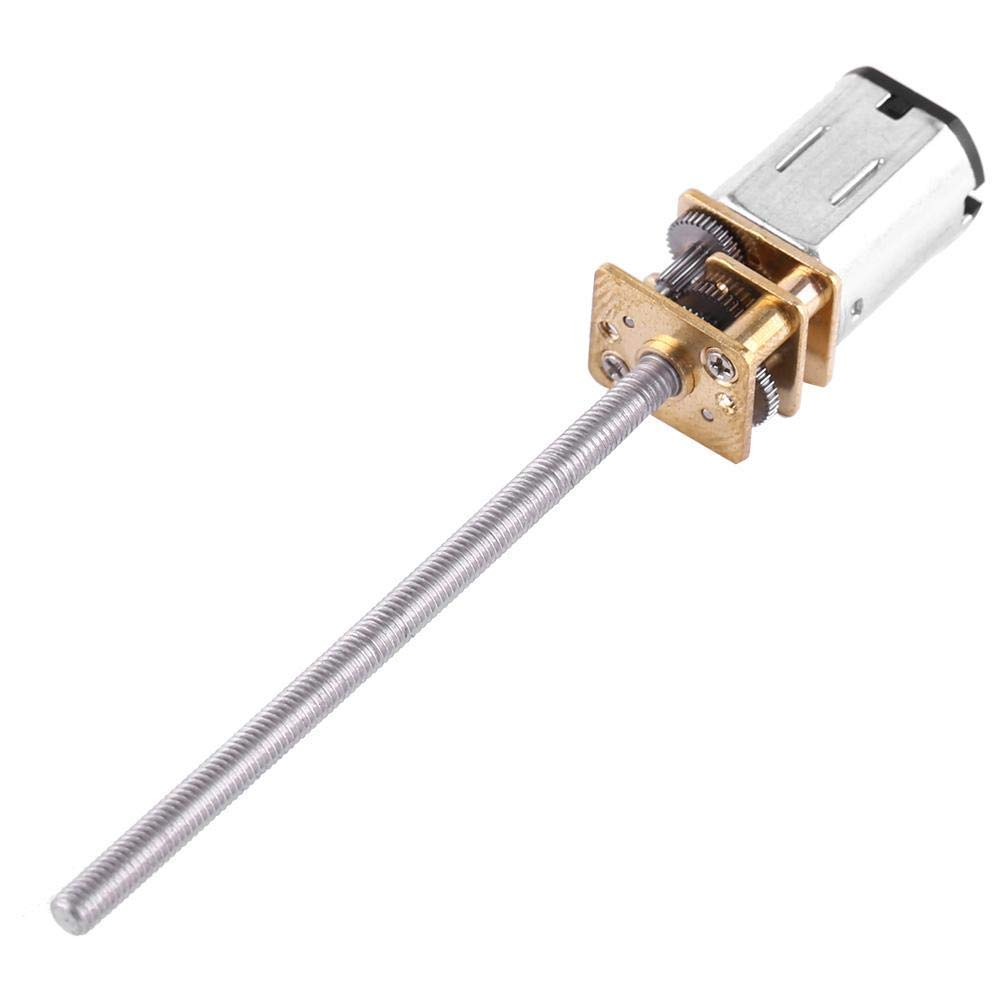
\includegraphics[width=\linewidth]{ImagenesMatriz/MotorEje.jpg}& 
		Mecanismo tornillo sinfin-corona curva \par\smallskip 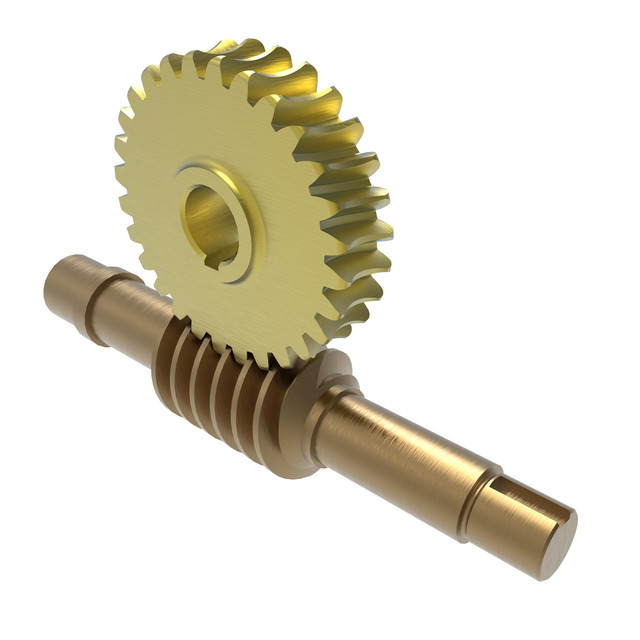
\includegraphics[width=\linewidth]{ImagenesMatriz/TornilloSinFinCorona.jpg}& 
		Transmisión por correa dentada \par\smallskip 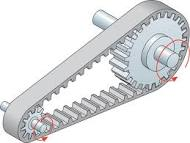
\includegraphics[width=\linewidth]{ImagenesMatriz/TransmisionCorreaDentada.jpg}\\ \hline
		\textbf{8. Posicionar plataforma} & 
		Soporte vertical  \par\smallskip 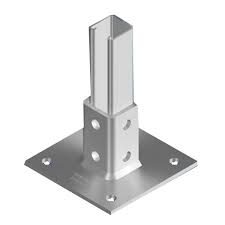
\includegraphics[width=\linewidth]{ImagenesMatriz/SoporteVertical.jpg}& 
		Plataforma elevadora de tijera \par\smallskip 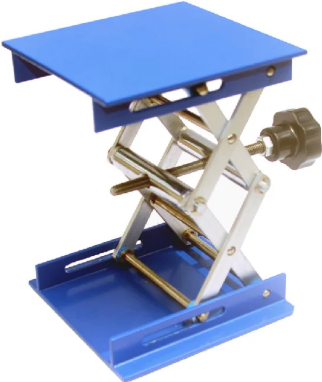
\includegraphics[width=\linewidth]{ImagenesMatriz/TijeraElevacion.png}& 
		Elevacion por articulación telescópica\par\smallskip 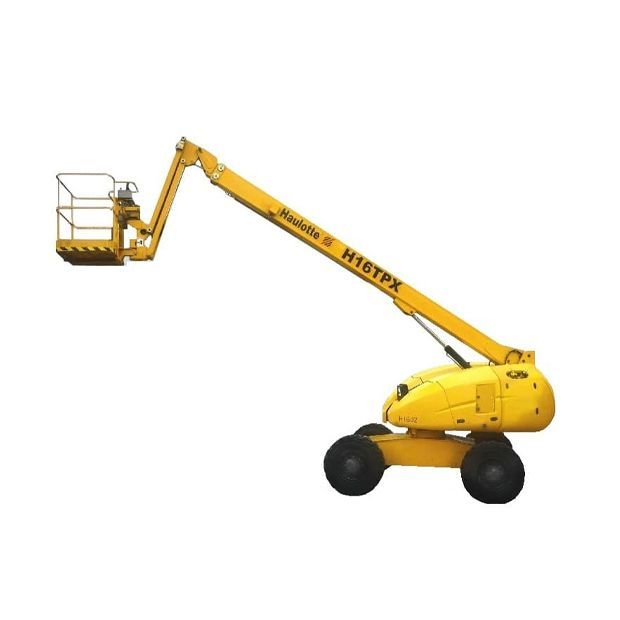
\includegraphics[width=\linewidth]{ImagenesMatriz/PlataformaTelescopica.jpg}\\ \hline
	\end{xltabular}
\end{center}

\begin{itemize}
	\item \textbf{Soportar plataforma de medición y Soportar componentes:} para conformar la estructura base, se evaluó el perfil V-Slot de aluminio, que ofrece una excelente relación resistencia-peso y gran modularidad para el ensamblaje; las chapas de acero, que brindan máxima rigidez estructural pero penalizan drásticamente el peso total del vehículo limitando su autonomía; y las piezas de MDF, una opción económica para prototipado rápido, pero mecánicamente frágil y vulnerable a la humedad del entorno exterior.
	
	\item \textbf{Proteger componentes, Alojar gestionador y Alojar memoria externa:} para el resguardo de la electrónica y módulos, se analizó la caja de chapa de aluminio, que proporciona ligereza, buena disipación térmica y resistencia natural a la corrosión; la caja de acero inoxidable, que garantiza una protección superior contra impactos y factores climáticos a cambio de un mayor costo y peso; y la carcasa impresa en 3D, ideal para geometrías complejas e integración a medida, pero con menor resistencia estructural a largo plazo frente a la radiación solar.
	
	\item \textbf{Generar movimiento de traslación:} para la movilidad del vehículo, se consideraron las ruedas con tracción de oruga, que aseguran un agarre óptimo y estabilidad sobre las superficies irregulares, zanjas o arena suelta comunes en las plantas solares, aunque demandan mayor consumo energético; la tracción diferencial de 4 ruedas, que resulta mecánicamente más simple y eficiente, pero es vulnerable a atascarse o patinar en terrenos blandos; y las ruedas omnidireccionales, que ofrecen máxima maniobrabilidad pero son inoperables en la topografía accidentada del campo.
	
	\item \textbf{Orientar plataforma:} para ajustar el ángulo de los instrumentos, se propuso el mecanismo de tornillo sinfín-corona curva, que destaca por su alta precisión y capacidad de retención estática (autobloqueo) para mantener la inclinación frente a las ráfagas de viento sin consumir energía continua; el eje acoplado a motor, que ofrece un diseño directo y simple pero exige torque constante del actuador para sostener la carga; y la transmisión por correa dentada, que permite movimientos rápidos pero es susceptible al desgaste, elongación y deslizamiento bajo condiciones de intemperie.
	
	 \item \textbf{Posicionar plataforma:} Se propuso el soporte vertical, que complementa el movimiento del motor lineal, pero puede sacrificar los grados de libertad para ajustar la orientación de la plataforma de medición; la plataforma elevadora de tijera, cuyos ejes mecánicos expuestos pueden resultar vulnerables al desgaste y atascamiento por el ingreso físico de polvo o arena del entorno; y la elevación por articulación telescópica, un principio tecnológico extraído de las actuales micro estaciones meteorológicas móviles \citep{CN222047271U}.

\end{itemize}